\documentclass[conference]{IEEEtran}
\IEEEoverridecommandlockouts
% The preceding line is only needed to identify funding in the first footnote. If that is unneeded, please comment it out.
%\usepackage{cite}
\usepackage[sorting=none]{biblatex}
\bibliography{bib}
\usepackage{amsmath,amssymb,amsfonts}
%\usepackage{algorithmic} % conflicts with algpseudocode (both define the algorithmic environment)
\usepackage{graphicx}
\usepackage{textcomp}
\usepackage{xcolor}
\usepackage{algorithm}
\usepackage{algpseudocode}
\setlength{\tabcolsep}{10pt} % Default value: 6pt
\renewcommand{\arraystretch}{1.5} % Default value: 1
\usepackage[skip=10pt]{caption}

\usepackage[caption=false,font=normalsize,labelfont=sf,textfont=sf]{subfig}
\def\BibTeX{{\rm B\kern-.05em{\sc i\kern-.025em b}\kern-.08em
    T\kern-.1667em\lower.7ex\hbox{E}\kern-.125emX}}
\begin{document}

\title{ISAR Reconstruction for Non-Uniform Sampling using Compressed Sensing Techniques}

%\author{\IEEEauthorblockN{1\textsuperscript{st} Given Name Surname}
%\IEEEauthorblockA{\textit{dept. name of organization (of Aff.)} \\
%\textit{name of organization (of Aff.)}\\
%City, Country \\
%email address or ORCID}
%\and
%\IEEEauthorblockN{2\textsuperscript{nd} Given Name Surname}
%\IEEEauthorblockA{\textit{dept. name of organization (of Aff.)} \\
%\textit{name of organization (of Aff.)}\\
%City, Country \\
%email address or ORCID}
%\and
%\IEEEauthorblockN{3\textsuperscript{rd} Given Name Surname}
%\IEEEauthorblockA{\textit{dept. name of organization (of Aff.)} \\
%\textit{name of organization (of Aff.)}\\
%City, Country \\
%email address or ORCID}
%\and
%\IEEEauthorblockN{4\textsuperscript{th} Given Name Surname}
%\IEEEauthorblockA{\textit{dept. name of organization (of Aff.)} \\
%\textit{name of organization (of Aff.)}\\
%City, Country \\
%email address or ORCID}
%\and
%\IEEEauthorblockN{5\textsuperscript{th} Given Name Surname}
%\IEEEauthorblockA{\textit{dept. name of organization (of Aff.)} \\
%\textit{name of organization (of Aff.)}\\
%City, Country \\
%email address or ORCID}
%\and
%\IEEEauthorblockN{6\textsuperscript{th} Given Name Surname}
%\IEEEauthorblockA{\textit{dept. name of organization (of Aff.)} \\
%\textit{name of organization (of Aff.)}\\
%City, Country \\
%email address or ORCID}
%}
\author{Brandon Boucher}
\maketitle

\begin{abstract}
Inverse Synthetic Aperture Radar (ISAR) imaging can form high resolution images of non-cooperative targets, but complex motion with higher-order motion terms can hinder standard image formation techniques. The Matching Fourier Transform is a popular method to form images of non-uniformly rotating targets as it compensates for the non-linear phase by incorporating the estimated motion parameters into the phase model \cite{Zuo_2020}. However, this method does not directly address non-uniform sampling. In order to produce high resolution images of targets with challenging motion, we propose that it may be beneficial to separate and optimize each individual image processing step, including non-uniform sampling correction, to improve overall performance. Compressed sensing enables image formation with sub-Nyquist sampling and has demonstrated an ability to reconstruct uniquely challenging images. This article formulates backprojection as an explicit linear system, demonstrates the effects of angular sampling density weighting compensating for non-uniform sampling and proposes a method using compressed sensing techniques for correcting non-uniform sampling and forming an image with super-resolution.
\end{abstract}

\begin{IEEEkeywords}
ISAR imaging, compressed sensing, non-uniform sampling
\end{IEEEkeywords}

\section{Introduction} \label{sec:intro}

% motivation
ISAR imaging enables image creation in all weather systems and is advantageous in many air-to-air and air-to-ground applications. The resolution of an ISAR image is dependent on the bandwidth of the radar and the rotation of the target. As the target rotates and the integration angle increases, the cross range resolution of the target improves. However, the motion of a target can be complex, complicating the image formation process and introducing undesirable deformations and artifacts. For instance, one application of ISAR imaging is to detect, classify and track missiles \cite{Liu_2012}. Some missiles like hypersonics not only move quickly, stressing motion compensation, but often employ a complex trajectory including rapid changes in translational and rotational acceleration in order to avoid detection and tracking. This complex motion can make image formation using standard techniques like Range-Doppler processing difficult. 

% introduce non-uniform sampling 
As a target rotates, each sample corresponds to a given angular change or angular sample. With a constant pulse repetition frequency (PRF), this angular sampling is constant for a uniformly rotating target. However, when angular acceleration is introduced, the corresponding angular sampling rate evolves over time. For a target starting from a stationary position and rotating with acceleration, the angular samples are dense at the beginning of the trajectory relative to the end. This is a result of the angular increment ($\Delta \theta_{k}$) increasing with increasing angular velocity for each sample ($k$). The non-uniformity in angular sampling deforms the point spread function (PSF) and the energy distribution in the spatial frequency domain where there is less energy within regions of sparse angular sampling. Figure \ref{fig:psf} depicts the deformation of the PSF for a point target for different angular accelerations, where the deformation amplifies with increasing angular acceleration. 

%This deformation in the PSF creates azimuth blurring and deformations in the sidelobes. Non-uniform sampling is a byproduct of non-uniform target rotation, and current methods account for the non-uniform sampling implicitly; however, addressing non-uniform sampling directly could improve image resolution and identification of non-cooperative targets.

\begin{figure*}[!t]
    \centering
    \subfloat[]{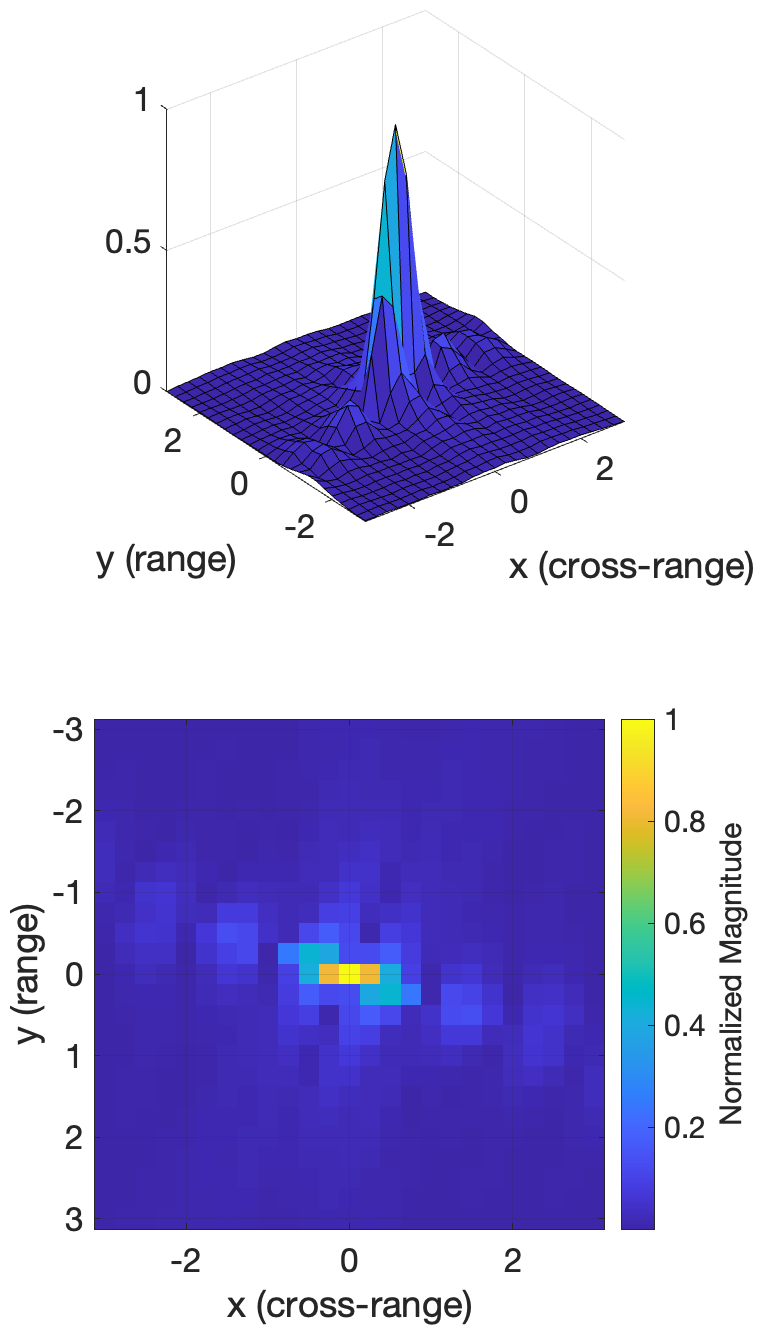
\includegraphics[width=0.3\linewidth]{Figures/psf_final_1.png}}%
    \label{fig:psf_a}
    \hfil
    \subfloat[]{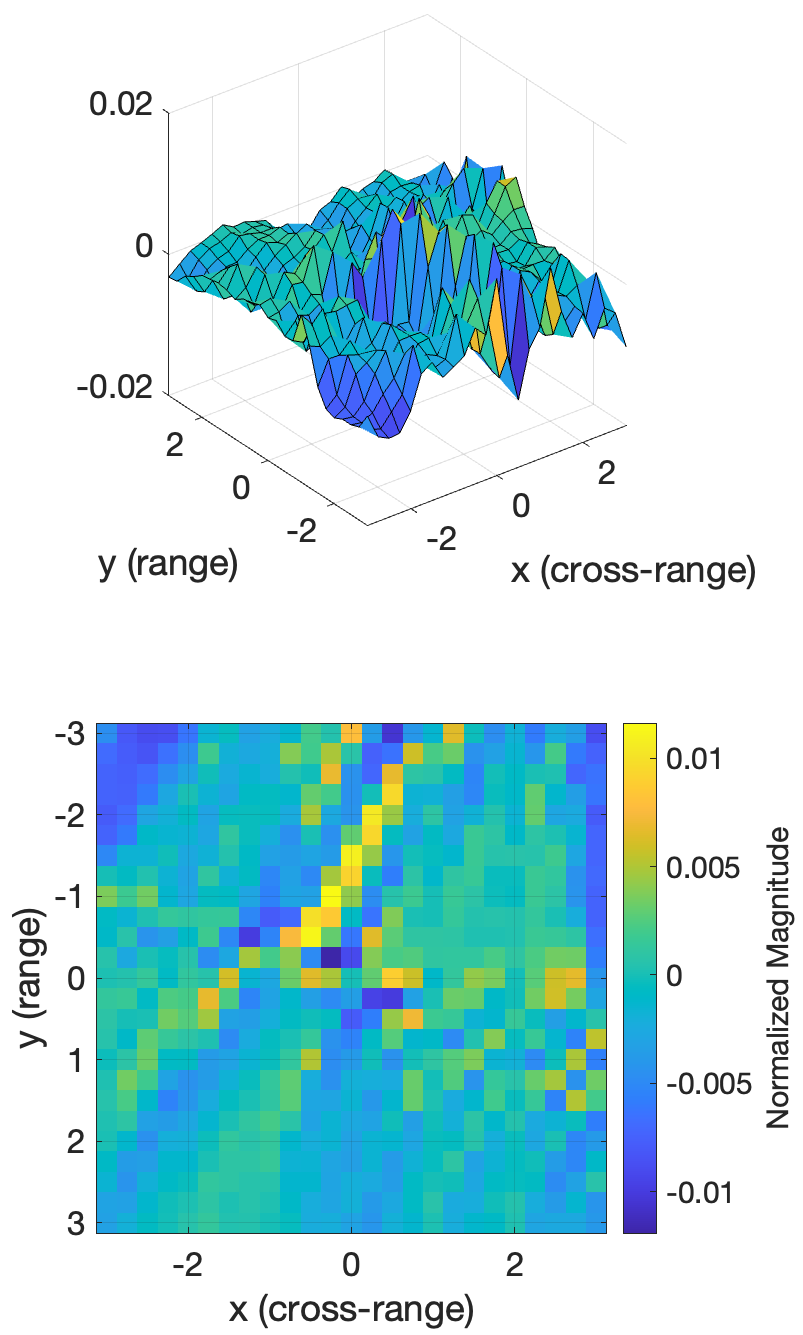
\includegraphics[width=0.3\linewidth]{Figures/psf_final_2.png}}%
    \label{fig:psf_b}
    \hfil
    \subfloat[]{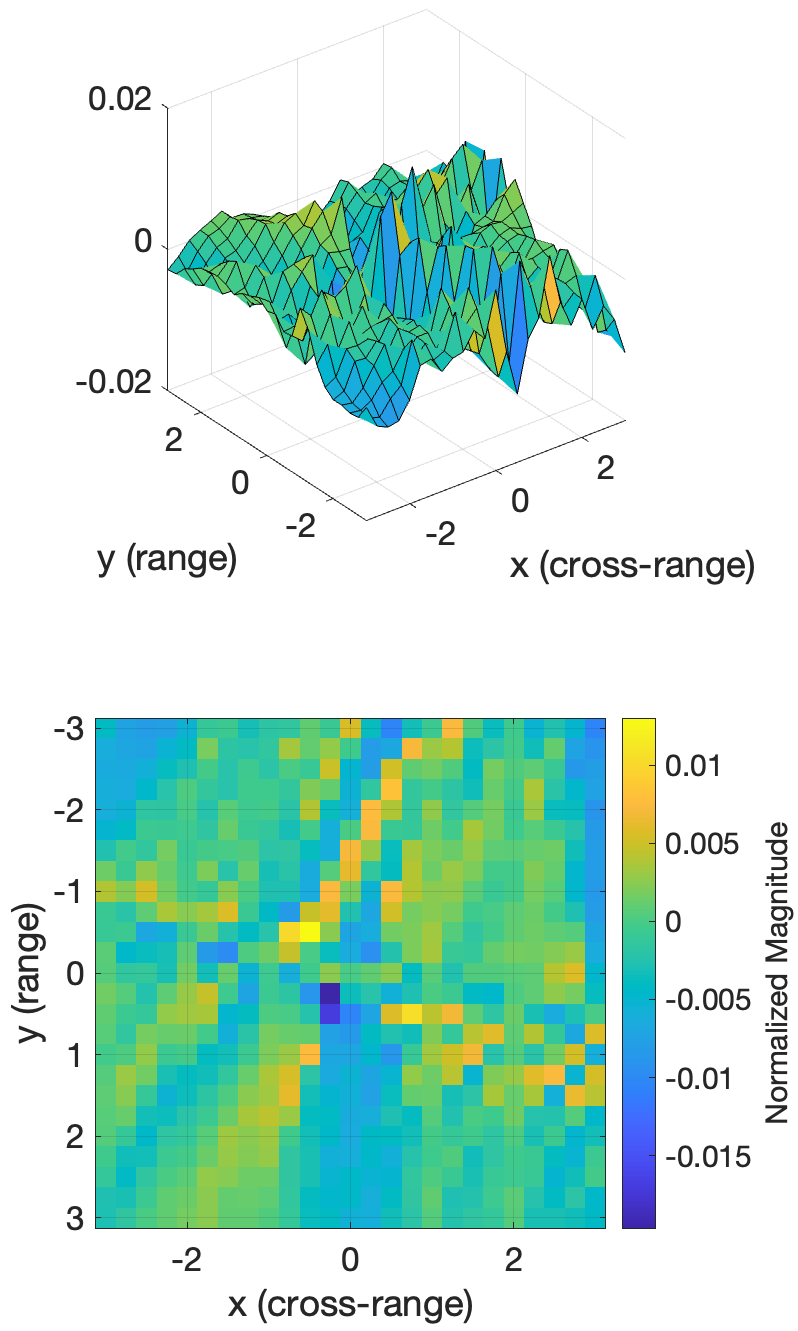
\includegraphics[width=0.3\linewidth]{Figures/psf_final_3.png}}%
    \label{fig:psf_c}
    \caption{Point spread function (PSF) for uniformly sampled target and target scatterers with non-uniform rotation. PSF for (a.) uniformly sampled target scatterer (b.) PSF difference of non-uniformly sampled image with $\dot{\omega} = \pi/4$ rad/s/s relative to uniformly sampled image (c.) PSF difference of non-uniformly sampled image with $\dot{\omega} = 2\pi$ rad/s/s relative to uniformly sampled image.}
\label{fig:psf}
\end{figure*}

% imaging for isar non-uniform target rotation
% vehmas_2016
% zhuo_2020

% compressed sensing
% Sun_2015
% Liu_2012

Recent literature regarding non-uniform rotation in ISAR imaging compensates for the image deformation from the perspective of optimally focusing the image \cite{Zuo_2020,Vehmas_2016}. In particular, the authors of \cite{Vehmas_2016} develop a procedure for optimally applying a range cell migration correction method and determining a kernel to apply in imaging a target with non-uniform rotation based on the contrast of the resulting ISAR image. The authors of \cite{Zuo_2020} have similar motivations by compensating for the target's angular acceleration by applying a matching Fourier transform (MFT), optimizing the image's quality by searching for the rotation ratio formed from the estimated motion parameters. Furthermore, other techniques incorporate compressed sensing assuming sparsity in a Fourier-domain \cite{Liu_2012, Sun_2015, Zhang_2019}. The methods in \cite{Liu_2012, Zhang_2019} improve image quality by incorporating rotational motion compensation in conjunction with a MFT basis with a randomly sampled measurement matrix. The authors in \cite{Sun_2015} construct a range-instantaneous Doppler sparsifying basis and solve an $l$-1 norm optimization problem to improve the image's clarity and reduce the noise level. These methods are effective in promoting a focused image, but do not directly address non-uniform sampling. By separating motion compensation, range cell migration correction and other processing techniques along with correcting for non-uniform sampling, each method can be optimized individually, potentially improving the resolution of the image.

There are many techniques for generally handling non-uniform sampling in SAR and ISAR. These methods have been derived for problems like SAR image formation in the near-field where the received data cannot be presumed to lie on a uniform Cartesian grid \cite{Subiza_2003} or as an extension of range cell migration correction where motion compensation to the center point of the scene leaves range migration for the non-center cells \cite{Meng_2015}. The principles in compensating for the curved grid for near-field imaging and for range cell migration are fundamentally the same problem, and the underlying methodology of solving these problems can be repurposed for imaging a non-uniformly rotating target. There are two primary imaging methods: frequency-based and time-based reconstruction. The standard frequency-domain domain methods require a uniform grid, necessitating the interpolation of the non-uniformly sampled grid. The time-based reconstruction methods like backprojection are equipped to resolve more challenging geometries including non-uniform sampling but require weighting based on the angular sampling. The modifications to the backprojection algorithm are often in combination with techniques aimed at improving computational efficiency.

% Fourier-based methods
% NuFFT
% gridding

Frequency-domain image formation techniques like Range-Doppler processing are advantageous for their computational efficiency but require more assumptions, including a uniformly sampled grid \cite{Malik_2005}. For an ISAR image of a non-uniformly rotating target, the non-uniformly sampled grid must be interpolated to a uniform grid prior to image formation \cite{Malik_2005}. There are several common methods for interpolating to a uniform grid: gridding, Stolt interpolation and non-uniform FFT (NuFFT)-based methods.

\begin{enumerate}
    \item Gridding interpolates data in the spatial frequency domain using a convolution function like a Gaussian, sinc function, nearest neighbor, etc \cite{Malik_2005,Jackson_1991, Pipe_1999}. The convolution function is convolved with the sampling density to weight samples uniformly, rectifying the deformation inherent to the k-space of a non-uniformly sampled image \cite{Malik_2005, Jackson_1991, Pipe_1999}. 
    \item $\Omega-k$ processing in combination with Stolt interpolation maps data in a non-uniform spatial-time domain to a uniform $\omega-k$ domain \cite{Meng_2015, Zhao_2018}. 
    \item The NuFFT transforms from non-uniform samples in the spatial-time domain to uniform samples in the spatial frequency domain (k-space) without explicit resampling or gridding \cite{Subiza_2003}.
\end{enumerate}

Backprojection is a time-domain method which coherently sums across pulses for each grid point to form an image. While considered computationally expensive relative to many Fourier-based methods, backprojection is often preferred in the context of challenging scenes as it requires less assumptions\cite{Zhang_2023}. Backprojection enables image formation on any defined grid and has been commonly used for mapping images onto three dimensional surfaces and reconstructing non-trivial tomography \cite{Ren_2009}. There are two common modified backprojection algorithm variants which correct for non-uniform sampling: filtered backprojection (FBP) and weighted backprojection (WBP):

\begin{enumerate}
    \item The FBP algorithm applies a ramp-filtering step in order to reducing the blurring resulting from non-uniform frequency weighting \cite{Zeng_2010, Zeng_2012, Zeng_2014} where the ramp-filtered backprojection can be determined by:
    
    \begin{equation}
        q(s, \theta) = p(s,\theta) *h(s)
    \end{equation}
    
    where $q(s,\theta)$ is the filtered output, $h(s)$ is the convolution kernel, $p(s,\theta)$ is the projected data, $\theta$ is an angle and $s$ is the spatial coordinate along the detector or crossrange axis \cite{Zeng_2010}. FBP has been used to address non-uniform sampling by defining a weighting matrix based on the radar parameters in the case of a non-uniform pulse repetition frequency in SAR imaging \cite{Tang_2016} and based on the geometry of the angular samples in the case of non-uniform sampling in MRI imaging \cite{Zeng_2012}. The weighting factor described in \cite{Zeng_2012} is defined using an angular density function $d(\theta)$:

    \begin{equation}
        b(i,j) = \left( \pi/\sum_{m=1}^{M} \frac{d(1)}{d(m)} \right) \sum_{m=1}^{M} \frac{d(1)}{d(m)} p(n,m) |_{INT}
    \end{equation}

    where $b$ is the backprojected image with an integration angle of $\pi$, $M$ is the total number of samples and $p$ is the projections interpolated at each angle $\theta$ \cite{Zeng_2012}.
    
    \item WBP has been used to address non-uniform sampling by similarly defining a weighting matrix which can be applied during or after backprojection \cite{Tang_2016, Grathwohl_2025}. In the case of applying weighting during backprojection for SAR imaging, the following weighting factor can be applied:
    
    \begin{equation}
        q(x) = \sum_{k=0}^{N - 1} W_{k}q_{k}(x)
        \label{eq:wbp}
    \end{equation}
    
    where $q$ is the final image, $q_{k}$ is the $k$-th sub-aperture or pulse of the backprojected image and $W_{k}$ is the weighting. Both the FBP and the WBP methods are fundamentally weighting the contributions of each pulse or sub-aperture based on the angular density of the sampling \cite{Tang_2016}.
\end{enumerate}

% fast + modified backprojection
Other approaches leverage the methodology inherent to the backprojection algorithm but speed up image formation by incorporating components of frequency-domain techniques. This can be seen in works like \cite{Zhao_2018}, where the authors transform from the non-uniform spatial-time domain to a uniform k-space using the NuFFT then integrate over the k-space, functionally performing a coherent summation. The authors from \cite{Meng_2015} first perform $\omega-k$ processing and Stolt interpolation, then apply a chirp modulation technique to built short apertures which can be coherently summed using backprojection. Backprojection is typically used as the foundation for addressing non-uniform sampling as its framework enables image formation for any geometry and is naturally conducive for imaging challenging target motion.

% linear systemizing for non-uniform sampling
% Zhang_2023
% compressed sensing for non-uniform sampling
% Bostock_2018
% Zobly_2011
Recently, new techniques have been developed to address non-uniform imaging by defining the system as a linear inverse problem. The authors in \cite{Zhang_2023} define a linear system emblematic of non-uniform signals, which is ill-posed. The sensing matrix is defined as a set of Fourier basis vectors with each entry in each basis vector corresponding to a non-uniform sample. The linear system's sampling rate is assumed to be greater than the Nyquist sampling rate and has a unique least squares solution, determined using Tikhonov regularization. Other methods define a signal or image with non-uniform sampling as a linear system and invoke compressed sensing techniques. The authors of \cite{Zobly_2011} and \cite{Bostock_2017} demonstrate the capability of applying a non-linear recovery process like the Greedy algorithms on a non-uniformly sampled measurement.

% novel contribution
This article forms an ISAR image using the time-domain backprojection algorithm in the framework of compressed sensing. The backprojection algorithm is used to construct an explicit linear system. This article depicts the effects of non-uniform sampling on an image formed with perfect motion compensation and applies angular sampling density weighting to the backprojection algorithm to improve the image quality, reducing the impact of the distorted sidelobes. The novel contribution of this article is introducing a methodology with the potential to improve image resolution by addressing the non-uniform sampling using compressed sensing techniques.

% article structure
The remainder of the introduction introduces the signal model and compressed sensing. Section II details the methodology and implementation of the formulation of the backprojection algorithm as an explicit linear system, the weighted backprojection algorithm and applying compressed sensing techniques to a non-uniform sampled signal. Section III contains the results, and Section IV and V contain the discussion and conclusion, respectively.

% ARCHIVE

%often rotational motion compensation is sufficient to focus the target scatterers in spatial domain. However, for higher resolution images and identification of non-cooperative targets, further refinement of the imaging process may be required to mitigate the sidelobes in the spatial domain and rectify the deformed PSF prevalent in the spatial frequency domain. 

%There are also a myriad of methods which combine different aspects of gridding, $\omega-k$ interpolation and the NuFFT, each with the intention of interpolating from a non-uniform grid to a uniform grid \cite{Zhao_2018}.

% Fourier-based methods

%Other methods incorporate the NuFFT to handle the non-uniform sampling in the frequency domain. This can be illustrated in performing $\omega-k$ processing. This range cell migration correction (RCMC) method transforms the spatial-time domain data to the $\omega-k$ domain then interpolating from a non-uniform grid to a uniform grid using the Stolt interpolation \cite{Meng_2015, Zhao_2018}. Other methods leverage the non-uniform FFT (NuFFT) to transform from the spatial-time domain to the spatial frequency domain (k-space). These methods have demonstrated promising results for common non-uniform sampling, enabling better computationally efficiency, but these techniques are likely insufficient for more challenging scenarios like the classification of hypersonic missiles.

% backprojection + weighted backprojection
%\indent Backprojection is a time-domain method which coherently sums across pulses for each grid point to form an image. Backprojection defines the imaging grid, naturally allowing flexibility in non-uniform sampling. In the context of non-uniform sampling, backprojection is typically used as it is able to produce high resolution images for any geometry, but it is computationally slow. Backprojection is able to project to any defined grid for any geometry by applying a phase correction dependent on the range each target scatterer for every pulse. However, this does not account for the deformation to the PRF. The sampling density deformation can be addressed by gridding, which interpolates from a non-uniform grid to a uniform grid and applies weighting based on the sampling density \cite{Pipe_1999, Malik_2005, Jackson_1991}. One method to address non-uniform sampling is to weight the backprojection, blah \cite{Tang_2016}

%Recent research leveraging backprojection seeks to speed up the image formation process in addition to interpolating the imaging grid. This can be accomplished by transforming from the non-uniform spatial-time domain to a uniform k-space using the NuFFT then integrating over the k-space, functionally performing a coherent summation \cite{Zhao_2018}. Other methods. First perform $\omega-k$ processing and Stolt interpolation, then apply a chirp modulation technique to built short apertures which can be coherently summed using backprojection.

%Other solutions include modifying the Pulse Repetition Frequency, hardware of the antenna, to account for the non-linear motion \cite{Moreira_1994}.  


\subsection{Signal model} \label{sec:signal}

\begin{figure}
    \centering
    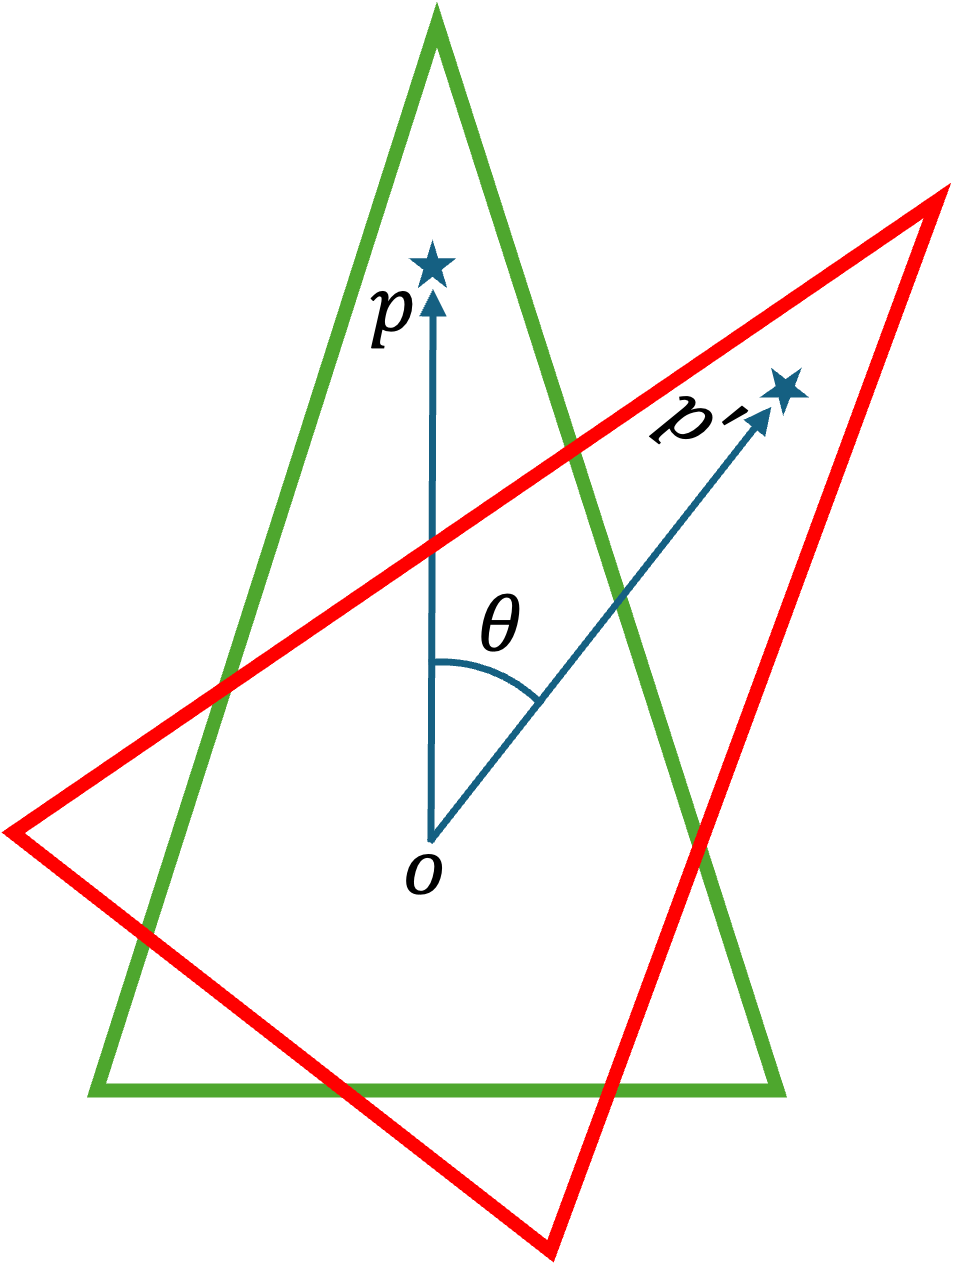
\includegraphics[width=0.4\linewidth]{target_geometry.png}
    \caption{ISAR Target Geometry}
    \label{fig:target_geometry}
\end{figure}

% target geometry
ISAR imaging requires translational motion compensation and rotational motion compensation. Translational motion compensation is typically regarded as trivial and does not add anything outside of undesirable blurring. Assuming the translational motion compensation has been appropriately applied, Figure \ref{fig:target_geometry} depicts the geometry of the target during ISAR imaging where the target is rotating $\Delta\theta$ between pulses. The signal can be represented as range compressed echo:

\begin{equation}
    s(t) = A\cdot \text{sinc}(B(\hat{t} - \tau))\cdot \exp(-j2 \pi f_{c} \tau)
\end{equation}

\noindent where $A$ is the amplitude, $B$ is the bandwidth, $\hat{t}$ is the fast time, $\tau$ is the propagation delay and $f_{c}$ is the center frequency. The propagation delay for a monostatic radar configuration is the amount of time required to propagate to the target and return:

\begin{equation}
    \tau = \frac{2R}{c}
\end{equation}

\noindent where $R$ is the range or distance from the radar to a target scattering point. The range for the geometry illustrated in Figure \ref{fig:target_geometry} can be defined as:

\begin{equation}
    R = R_{0} + x_{p} \cos(\theta(t)) + y_{p}\sin(\theta(t))
\end{equation}

\noindent where $R_{0}$ is the distance from the radar to the rotational axis of the target or $O$ from Figure \ref{fig:target_geometry}, $\theta(t)$ is the angle as a function of the slow time $t$, $x_{p}$ and $y_{p}$ are the distances along the x-axis and y-axis from the axis rotation to the scattering point $P$, respectively. Assuming a start-stop approach to modeling the angle, where the angle is assumed constant over the duration of the pulse's propagation to the target and back, the angle model can be defined as a Taylor series:

\begin{equation}
    \theta(t) \approx \theta(0) + \omega t + \frac{1}{2}\alpha t^{2}
\end{equation}


\subsection{Compressed sensing} \label{sec:cs}

Compressed sensing is a methodology that reconstructs images sampled below the Nyquist sampling rate, relying on the sparsity of the latent image. To understand the underlying formulation of compressed sensing, begin with a linear system:

\begin{equation}
    y = Ax
    \label{eq:yAx}
\end{equation}

\noindent where $y \in \mathbb{C}^{M}$ is the measurement, $x \in \mathbb{C}^{N}$ is the latent signal and $A$ is the sensing matrix. In most instances of compressed sensing, the length of the measurement is significantly less than the length of the latent signal ($M << N$). The system is underdetermined and has infinitely many solutions, each existing in the ($N-M$)-dimensional null space of the sensing matrix. However, if the latent image can be assumed $K$-sparse or containing $K$ non-zero values, the problem becomes $K$-dimensional where $M \geq K$. Additionally, if the sensing matrix is roughly orthogonal and incoherent, associated with the Restricted Isometric Property (RIP), the solution can be unique \cite{Majumdar_2018}. The compressed sensing problem can then be formulated as:

\begin{equation}
    \min_{x} ||x||_{0} \quad \text{subject to} \quad y = Ax
    \label{eq:l0}
\end{equation}

However, Equation \ref{eq:l0} is NP-hard and it is more computationally efficient to solve the convex problem \cite{Majumdar_2018}:

\begin{equation}
    \min_{x} ||x||_{1} \quad \text{subject to} \quad y = Ax
\end{equation}

This and variants of this problem are the foundation of what compressed sensing seeks to solve. The formulation of the problem relies on defining the sensing matrix. The sensing matrix is constructed as a combination of a sparsifying transformation ($\psi$) and a measurement matrix ($\phi$) such that:

\begin{equation}
    A = \Phi \Psi
    \label{eq:A}
\end{equation}

There are many different compressed techniques, and Greedy algorithms like Orthogonal Matching Pursuit (OMP) are effective for non-linear recovery \cite{Bostock_2017}. For a Hermitian sensing matrix ($A$) where $A^{-1} = A^{H}$, OMP iterates through a defined sparsity ($K$) and finds the indices ($\Lambda$) that maximize the projection of the residual, initialized as the measurement, onto the basis vectors formed by $A$. The maximization of the residual selects the coefficients projected on the basis vectors formed by $A$, and the step $r = y - A \hat{X}$ prevents the re-selection of the same indices. The latent image estimation $\hat{X}$ is the least-squares approximation formed from the selected basis vectors of $A$. Algorithm \ref{algo:OMP} formally describes the OMP algorithm \cite{Majumdar_2018}.



\begin{algorithm}[H]
\caption{Orthogonal Matching Pursuit}\label{algo:OMP}
\begin{algorithmic}[1]
\Procedure{OMP}{$H,N$}
\State $\Lambda\gets []$
\State $r \gets y$
\State $\hat{X} \gets 0$
\For{$i \leq K$}
\State $c\gets A^{H}r$
\State $\Lambda = \arg\max_{i} \big| c_i \big|$
\State $\Lambda \gets \begin{bmatrix} \Lambda \\ l \end{bmatrix}$
\State $\hat{X} \gets (A(\Lambda)^{H}A(\Lambda))^{-1}A(\Lambda)^{H}y$
\State $r \gets y - A\hat{X}$
\State $i \gets i + 1$
\EndFor
\State \textbf{return} $\hat{X}$
\EndProcedure
\end{algorithmic}
\end{algorithm}

% greedy algorithms / OMP?

\begin{figure*}[ht]
    \centering
    \subfloat[]{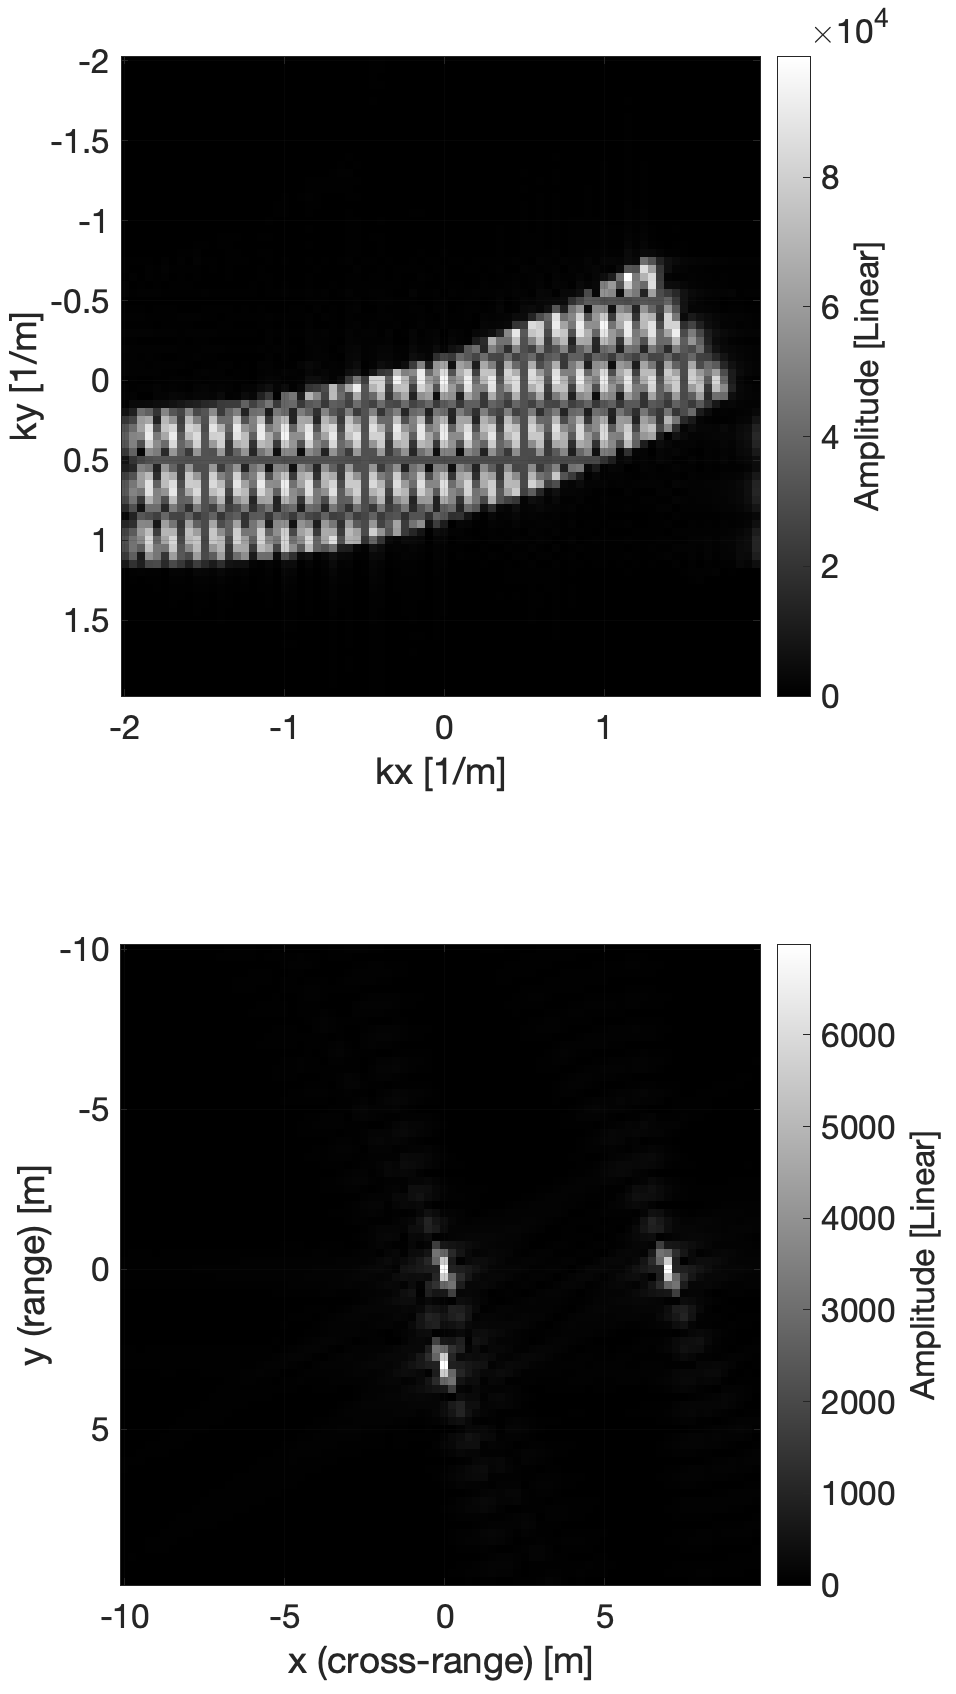
\includegraphics[width=0.23\linewidth]{Figures/sd_sfd_0.png}}%
    \label{fig:sd_sfd_a}
    \hfil
    \subfloat[]{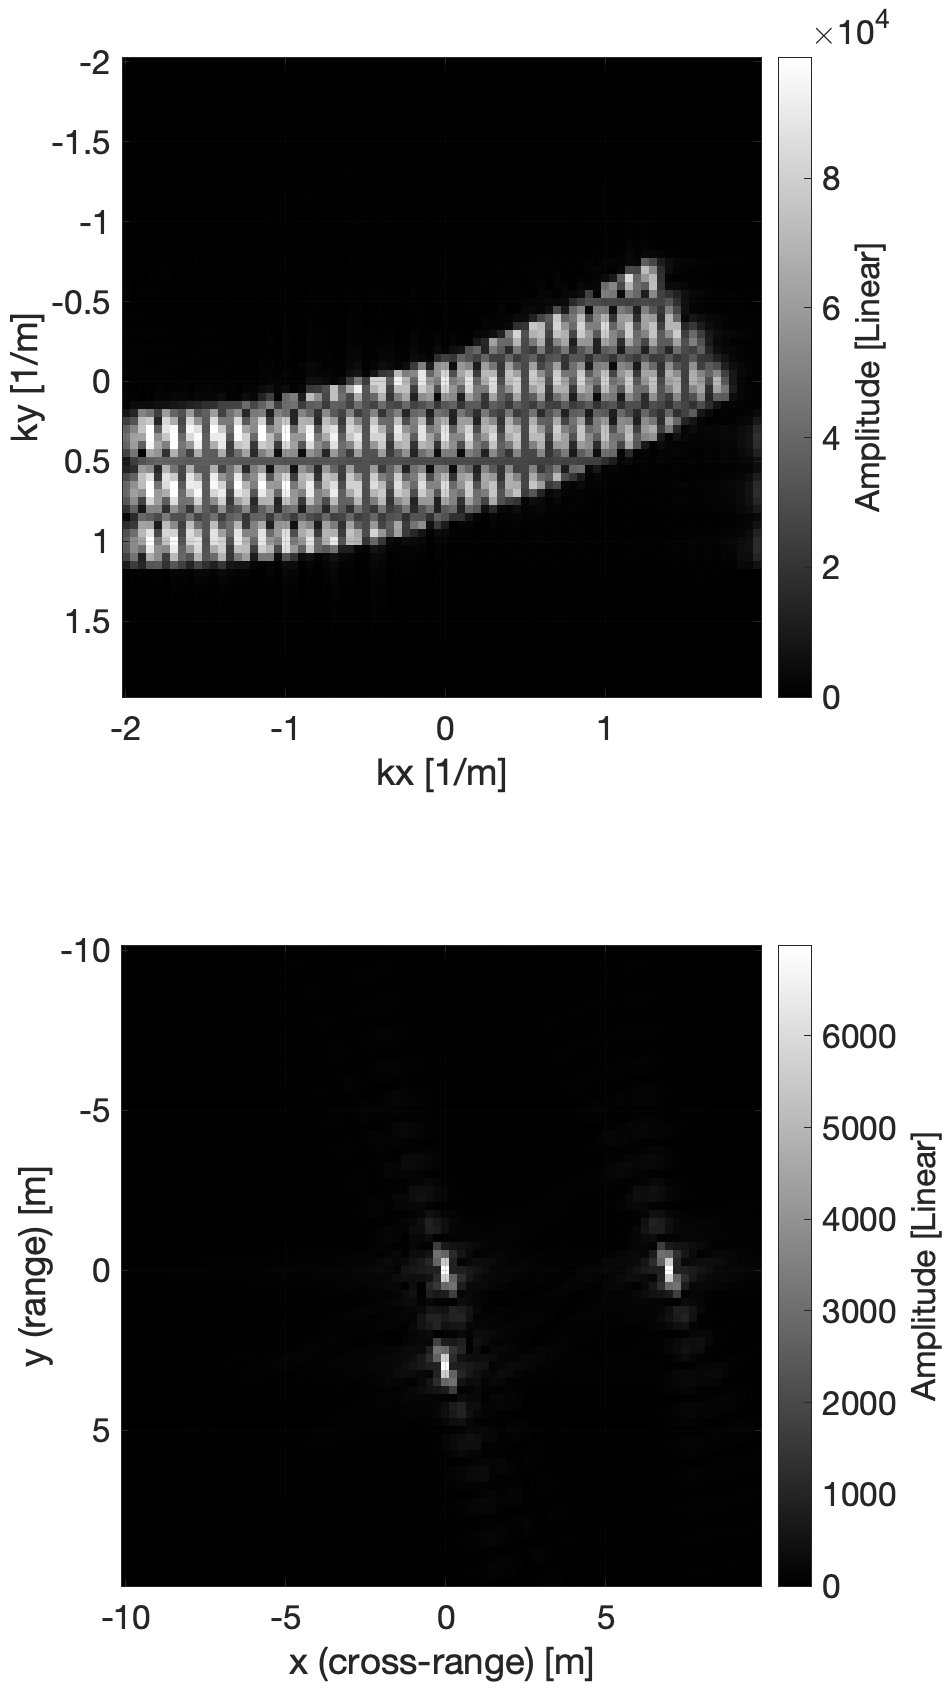
\includegraphics[width=0.23\linewidth]{Figures/sd_sfd_8.png}}%
    \label{fig:sd_sfd_b}
    \hfil
    \subfloat[]{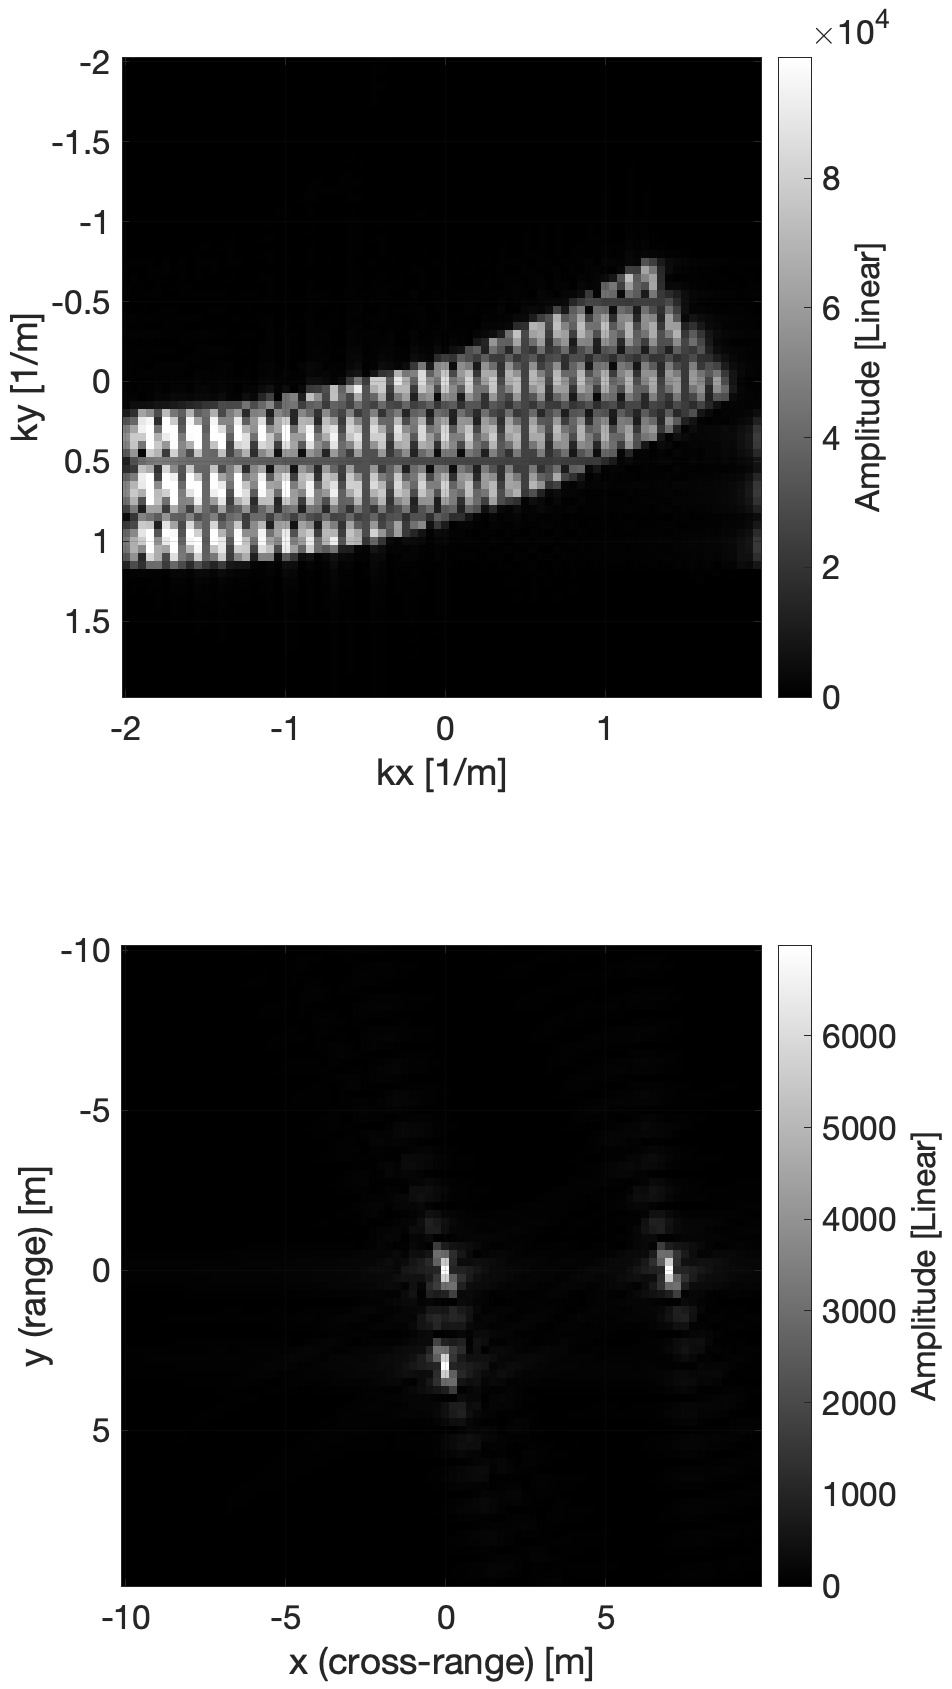
\includegraphics[width=0.23\linewidth]{Figures/sd_sfd_4.png}}%
    \label{fig:sd_sfd_c}
    \hfil
    \subfloat[]{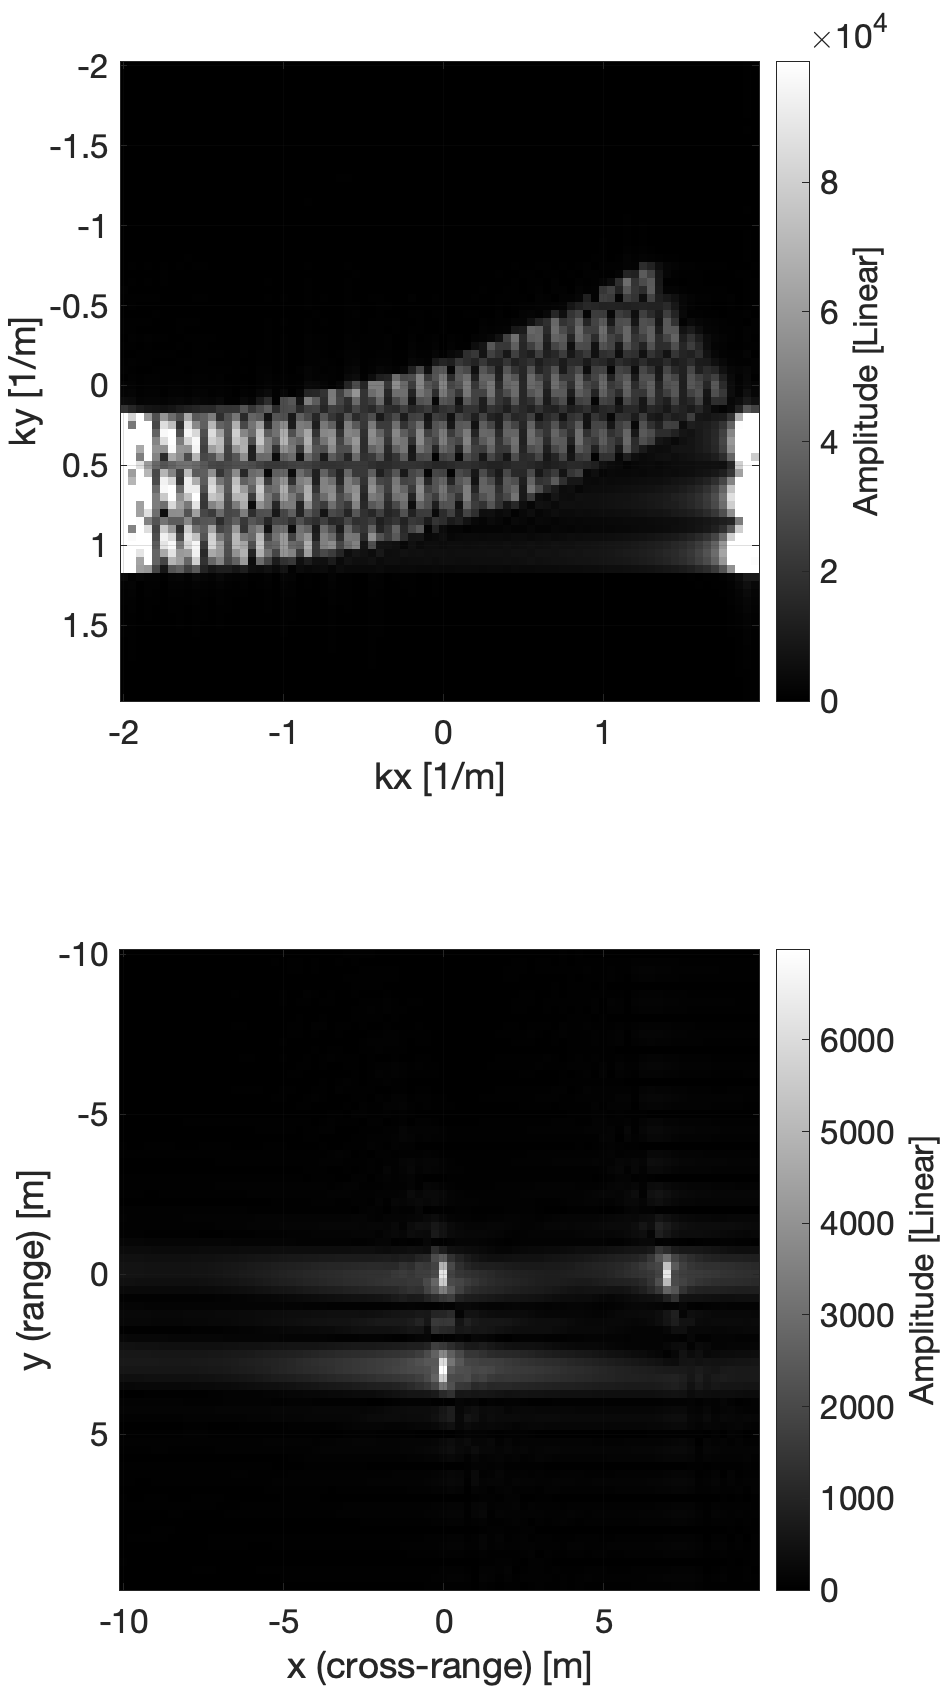
\includegraphics[width=0.23\linewidth]{Figures/sd_sfd_1.png}}%
    \label{fig:sd_sfd_d}
    \hfil
    \caption{ISAR imaging using standard backprojection of a rotating target with three scatterers in the (top) spatial frequency domain and (bottom) spatial domain with angular acceleration (left to right) of $0$ rad/s/s, $\pi/8$ rad/s/s, $\pi/4$ rad/s/s and $\pi$ rad/s/s.}
\label{fig:sd_sfd}
\end{figure*}

\section{Methods} \label{sec:methods}

This section will review the methodology of forming an ISAR image of a non-uniformly rotating target, directly addressing non-uniform sampling. Section \ref{sec:bp_la} reviews the reformulation of the backprojection algorithm into an explicit linear system. Section \ref{sec:wbp} discusses the modifications to the backprojection algorithm required to address non-uniform sampling using angular sampling density weighting. Section \ref{sec:bp_cs} discusses reconstruction using the principles described in Section \ref{sec:cs}. 

\subsection{Representing backprojection as an explicit linear system} \label{sec:bp_la}

There are several standard image formation techniques used for ISAR imaging as discussed in Section \ref{sec:intro}. The Fourier-based methods are more computationally efficient but often assume well-behaved linear target motion. For targets with complex motion, the backprojection algorithm is more suitable as it is adaptable in compensating for maneuvering targets, and for that reason this article will reconstruct using the backprojection algorithm.

To leverage the capabilities of compressed sensing, it is advantageous to formulate the ISAR image formation process to mirror the linear system defined in Equation \ref{eq:yAx}. The measurement ($y$) is the raw ISAR data formed using the methodology described in the signal model Section \ref{sec:signal}, and the latent image ($x$) is the desired focused image. In the case of a couple of target scatterers, the image domain is sufficiently sparse. From Equation \ref{eq:A}, the sparsifying transform ($\psi$) will reflect the backprojection algorithm where the adjoint of the focused image is formed by interpolating from the phase history to a defined grid ($\psi_{in}$), and the signal is coherently summed across all pulses ($\psi_{bp}$) \cite{Focsa_2021, Bonfert_2024}. The sparsifying transformation can then be defined as:

\begin{equation}
    \Psi = \Psi_{bp} \Psi_{in}
\end{equation}

The phase history data, $y \in  \mathbb{C}^{N_{r} \times N_{p}}$, where $N_{r}$ is the number of range bins and $N_{p}$ is the number of pulses, is transformed into an image $x = \mathbb{C}^{N_{x} \times N_{y}}$ where $N_{x}$ and $N_{y}$ are the number of grid points along the x-axis and y-axis, respectively. The sensing matrix formation process can be described as \cite{Focsa_2021}: 

\begin{enumerate}
    \item Find the distance from the radar at the origin $(0,0,0)$ to each grid point $(i,j)$ for each pulse ($p$): 
    \begin{equation}
        r_{ij}^{p} = \sqrt{x_{ij}^{2} + y_{ij}^{2} + z_{ij}^{2}}
    \end{equation}
    \item Truncate the evaluated ranges from the minimum to the maximum $r_{ij}^{p}$.
    \item Create a grid interpolation matrix ($\Psi_{in}$) with size $N_{x}\cdot N_{y} \cdot N_{p} \times N_{r}$ containing linear interpolation weights between the range cells containing the grid point at each pulse. The index of the constraining range cells can be found by:
    \begin{equation}
        k_{1,2} = \min_{k} |r - r_{ij}^{p}|
    \end{equation}
    \noindent where $r \in \mathbb{R}^{N_{r}}$ is an array of range values defined by fast time array. The $\Psi_{in}$ can therefore be defined as \cite{Focsa_2021}:
    
    \begin{equation}
        \begin{aligned}
            \psi_{in}^{p}(i,j,k_{1}) &= 1-\left[ \frac{r_{ij}^{p} - r(k_{1})}{r(k_{2}) - r(k_{1})} \right]\\
            \psi_{in}^{p}(i,j,k_{2}) &=1-\left[\frac{r(k_{1}) - r_{ij}^{p}}{r(k_{2}) - r(k_{1})} \right]
        \end{aligned}
    \end{equation}

    \item Create the azimuth suppression matrix ($\Psi_{bp}$) with size $N_{x} \cdot N_{y} \times N_{x} \cdot N_{y} \cdot N_{p}$ where the phase correction for each pulse is defined as:
    \begin{equation}
        \phi^{p}(r_{ij}^{p}) = \exp(j4\pi f_{c} r_{ij}^{p})
    \end{equation}
\end{enumerate}

The combination of the grid interpolation matrix and the azimuth suppression matrix applied to the measurement ($y$) forms the image-domain backprojected latent image ($x$)

\begin{equation}
    \begin{aligned}
        x &= A^{-1}y \\
         &= A^{H}y\\
         &= \Psi_{bp} \Psi_{in} y
    \end{aligned}
    \label{eq:Ah}
\end{equation}



\begin{figure*}[ht]
    \centering
    \subfloat[]{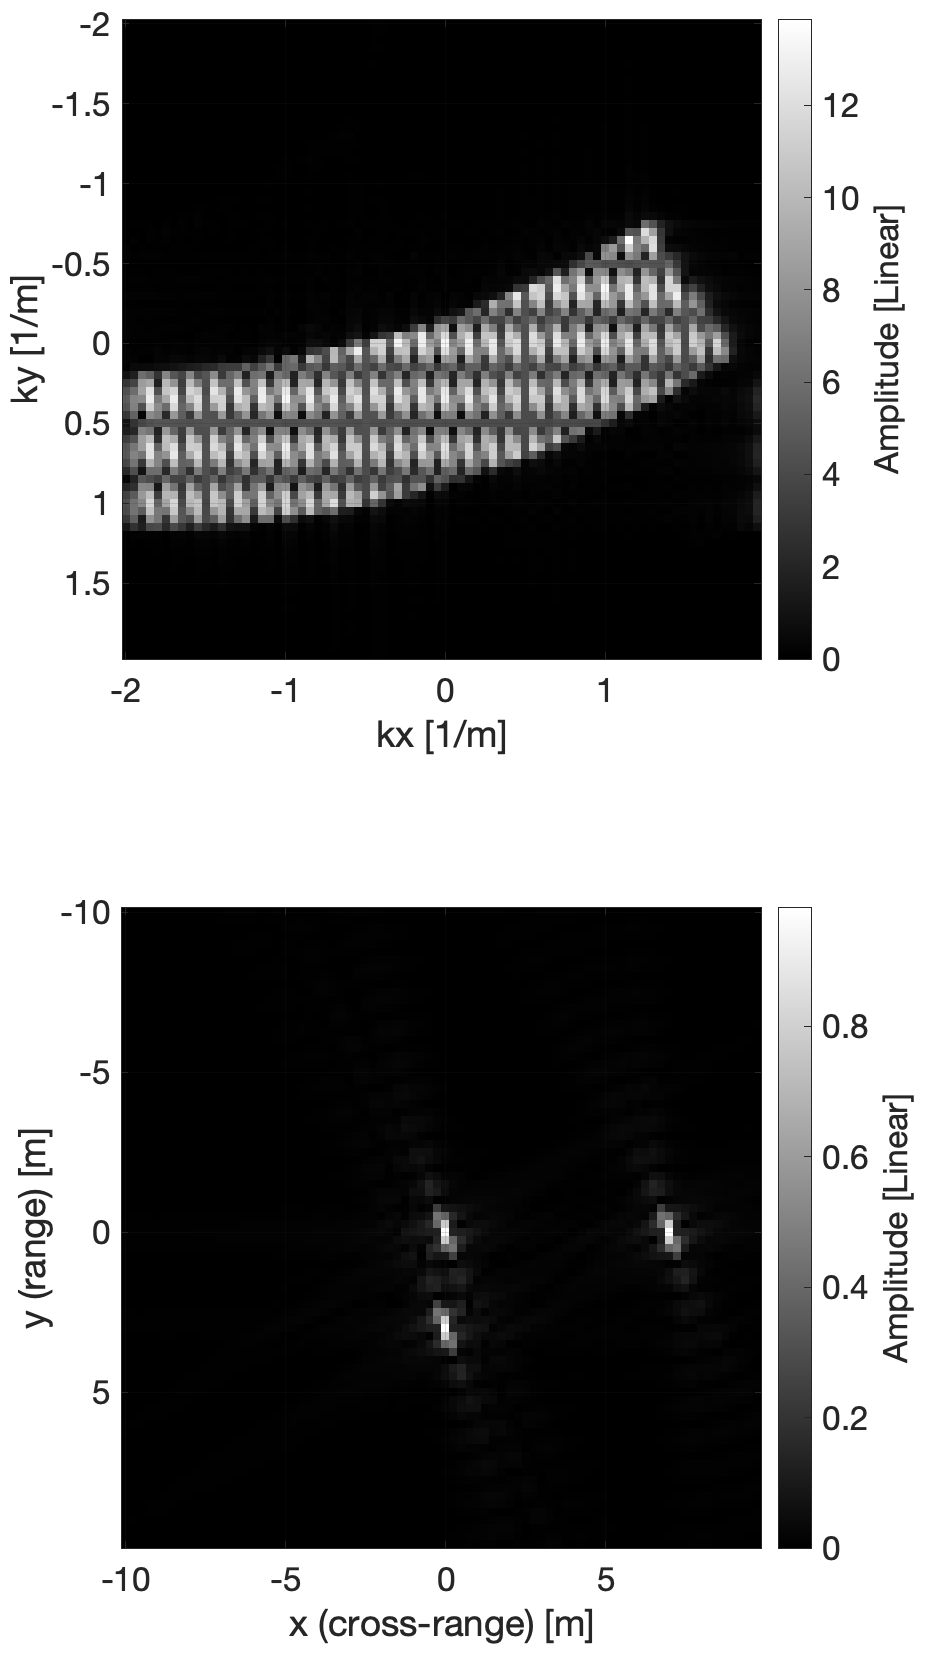
\includegraphics[width=0.23\linewidth]{Figures/sd_sfd_0_w.png}}%
    \label{fig:sd_sfd_a}
    \hfil
    \subfloat[]{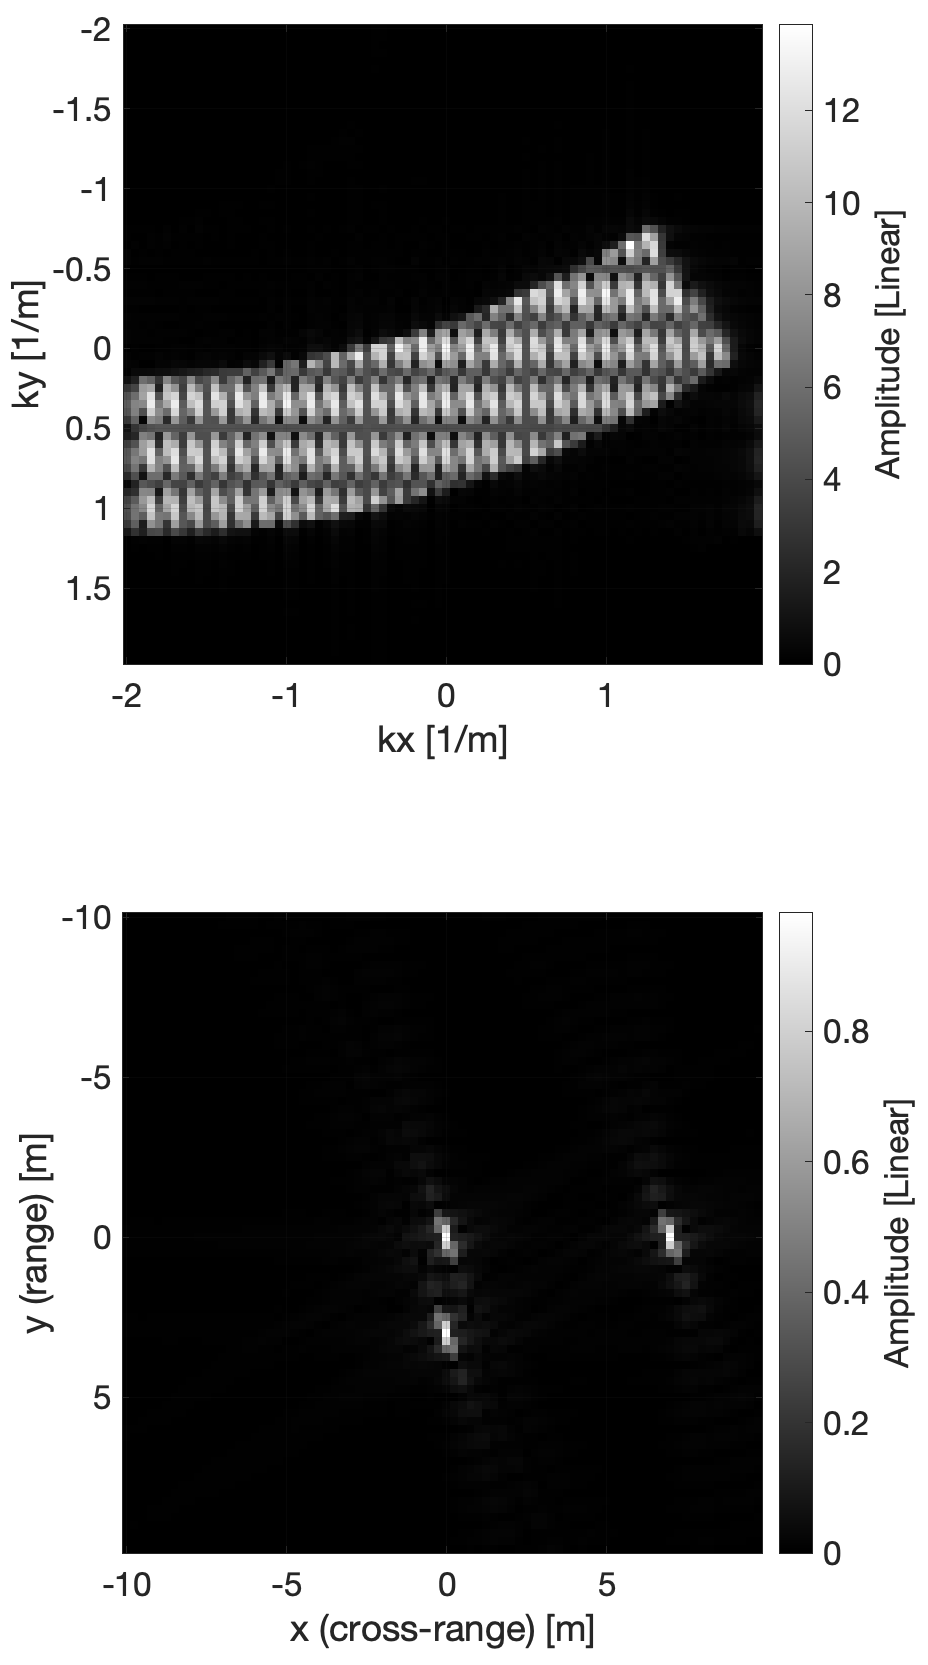
\includegraphics[width=0.23\linewidth]{Figures/sd_sfd_8_w.png}}%
    \label{fig:sd_sfd_b}
    \hfil
    \subfloat[]{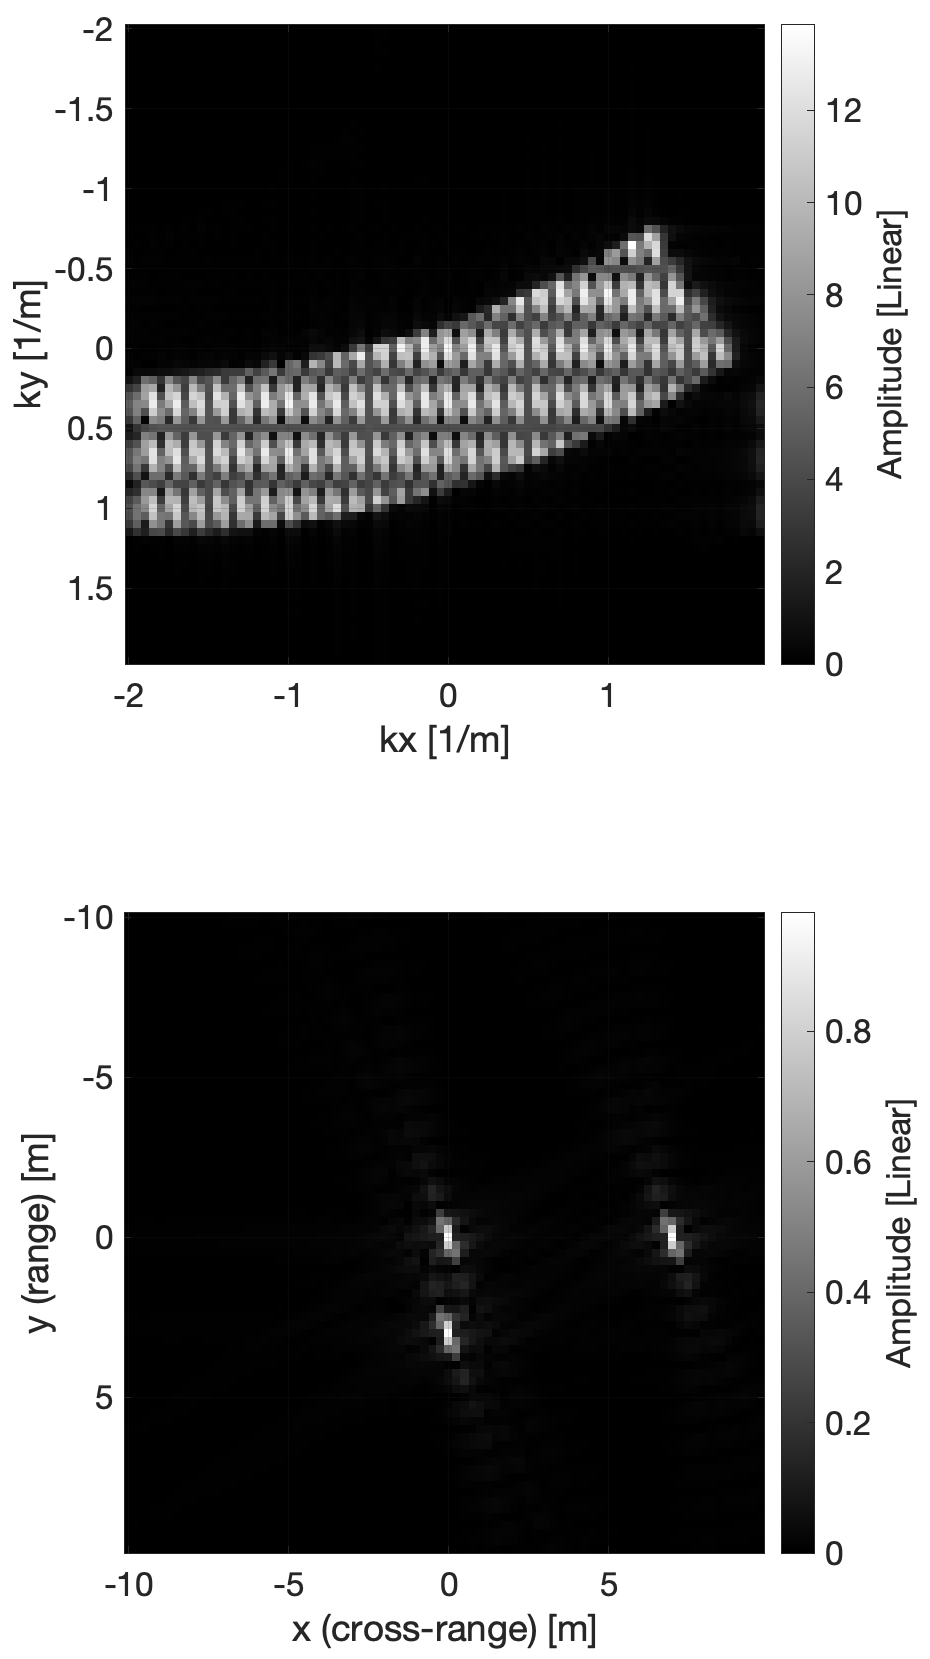
\includegraphics[width=0.23\linewidth]{Figures/sd_sfd_4_w.png}}%
    \label{fig:sd_sfd_c}
    \hfil
    \subfloat[]{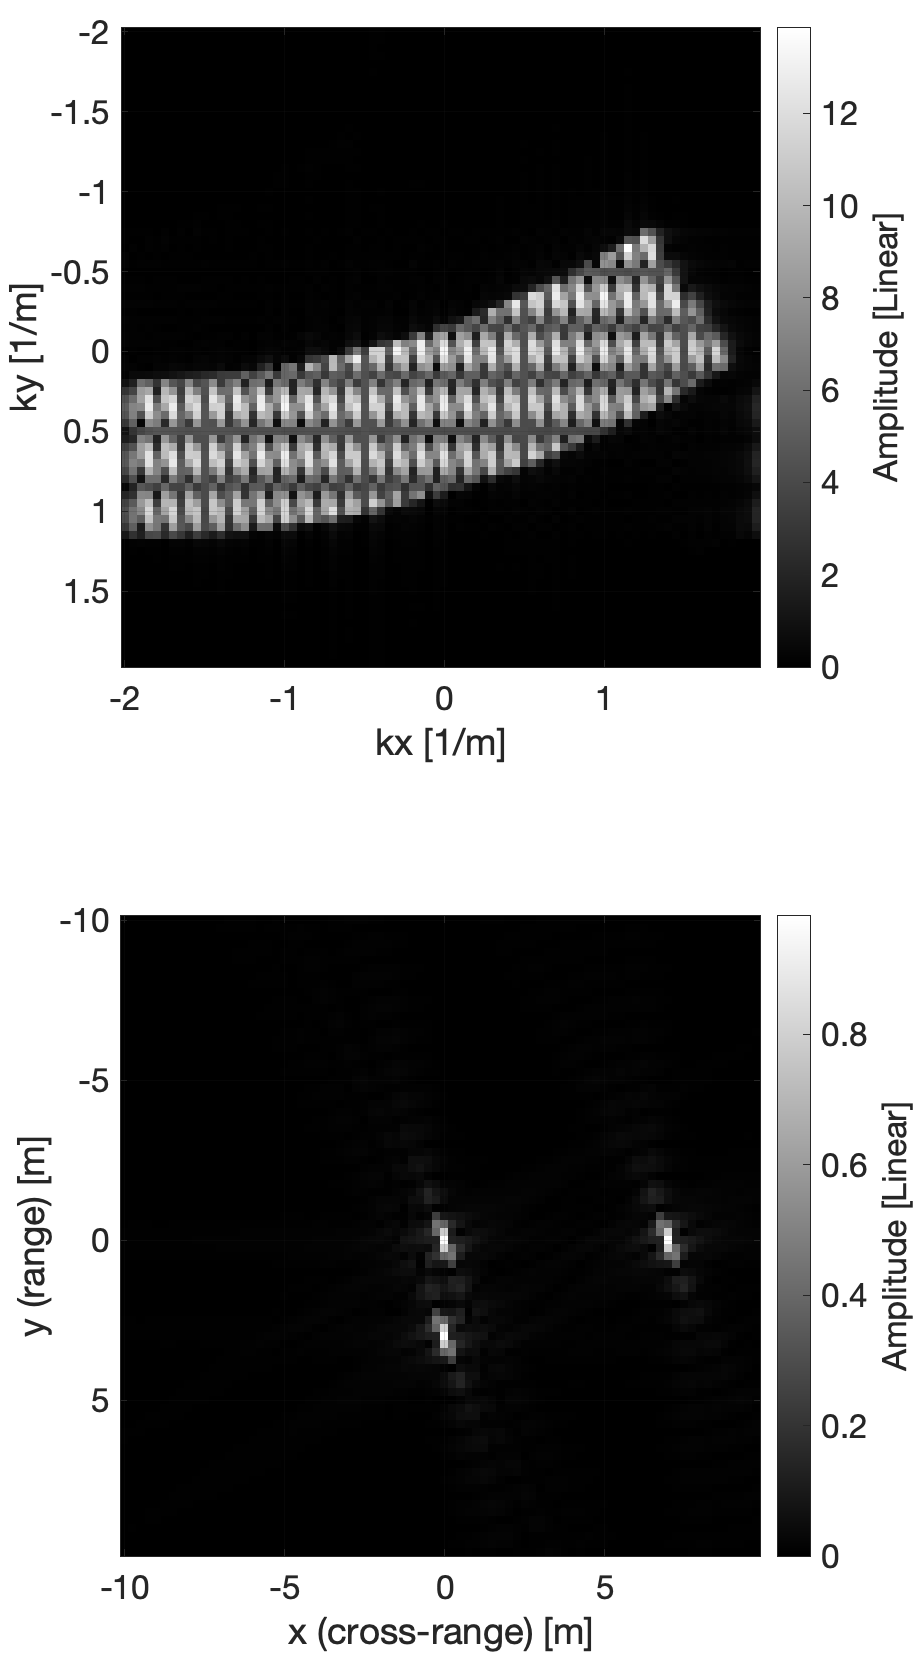
\includegraphics[width=0.23\linewidth]{Figures/sd_sfd_1_w.png}}%
    \label{fig:sd_sfd_d}
    \hfil
    \caption{ISAR imaging using weighted backprojection as described in Section \ref{sec:wbp} of a rotating target with three scatterers in the (top) spatial frequency domain and (bottom) spatial domain with angular acceleration (left to right) of $0$ rad/s/s, $\pi/8$ rad/s/s, $\pi/4$ rad/s/s and $\pi$ rad/s/s.}
\label{fig:sd_sfd_w}
\end{figure*}

\begin{figure*}[ht]
    \centering
    \subfloat[]{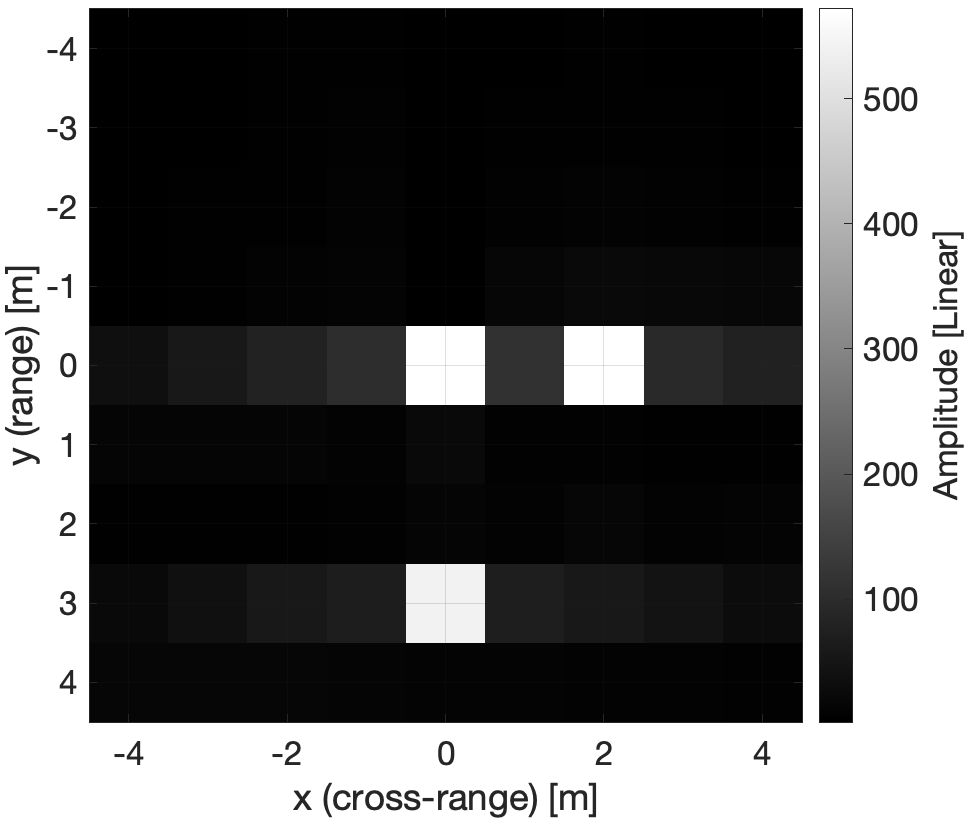
\includegraphics[width=0.3\linewidth]{Figures/backproj_la.png}}%
    \label{fig:backproj_la}
    \hfil
    \subfloat[]{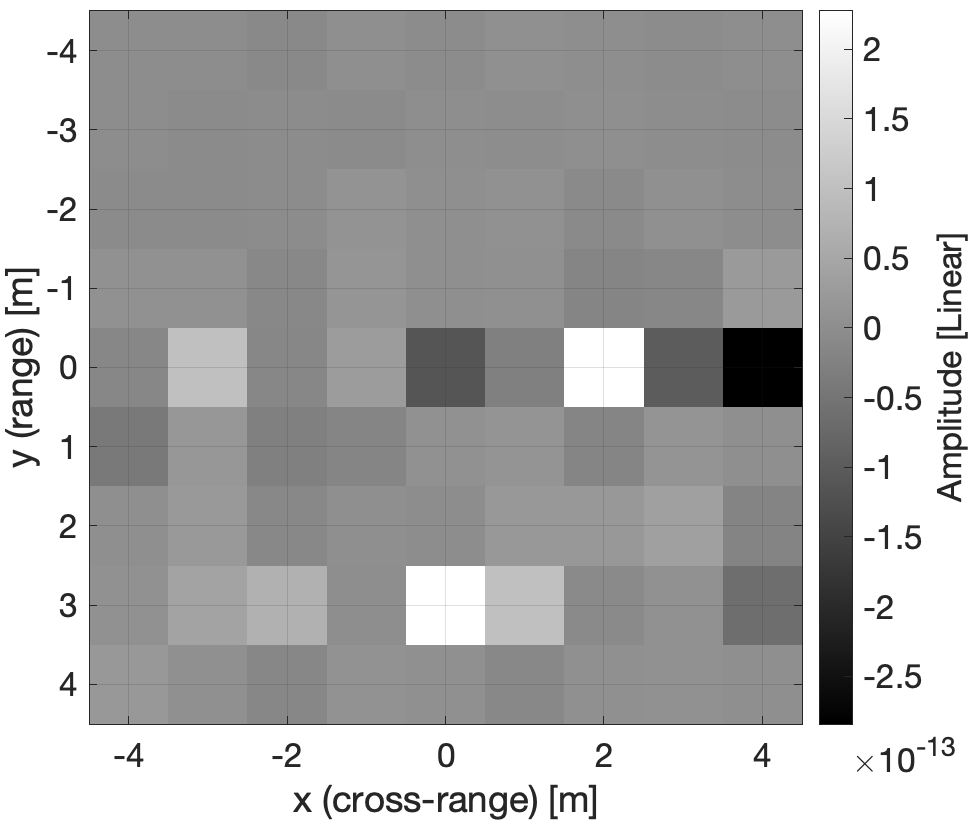
\includegraphics[width=0.3\linewidth]{Figures/backproj_la_diff.png}}%
    \label{fig:backproj_la_diff}
    \hfil
    \caption{ISAR imaging of a rotating target with scatterers at (1000,0), (1000, 2) and (1003, 0) with an angular velocity of $\omega = \pi$ rad and an integration angle of $10^{\circ}$. The radar parameters are reflected in Table \ref{tab:radar}, and the imaging pixel resolution is set to 1 meter in both the x-direction and in the y-direction. (a.) An image formed using backprojection algorithm re-formulated into a linear system and (b.) the difference between the standard backprojection algorithm and the backprojection algorithm formulated from Section \ref{sec:bp_la}.}
\label{fig:bp_la}
\end{figure*}

\begin{figure*}[ht]
    \centering
    \subfloat[]{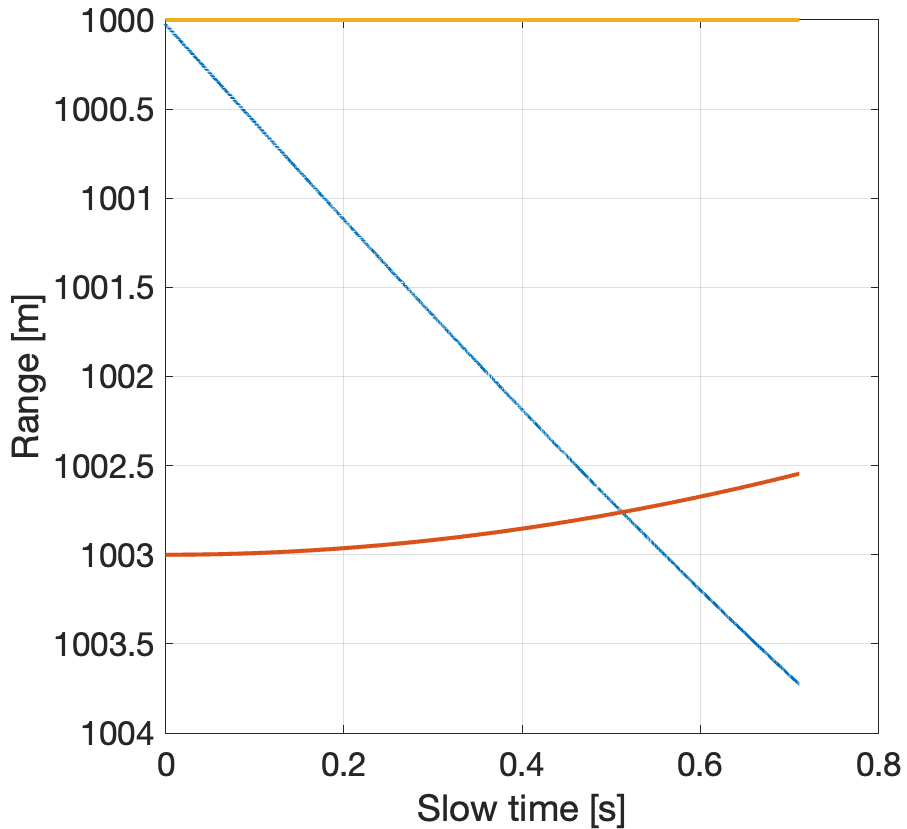
\includegraphics[width=0.3\linewidth]{Figures/range.png}}%
    \label{fig:range}
    \hfil
    \subfloat[]{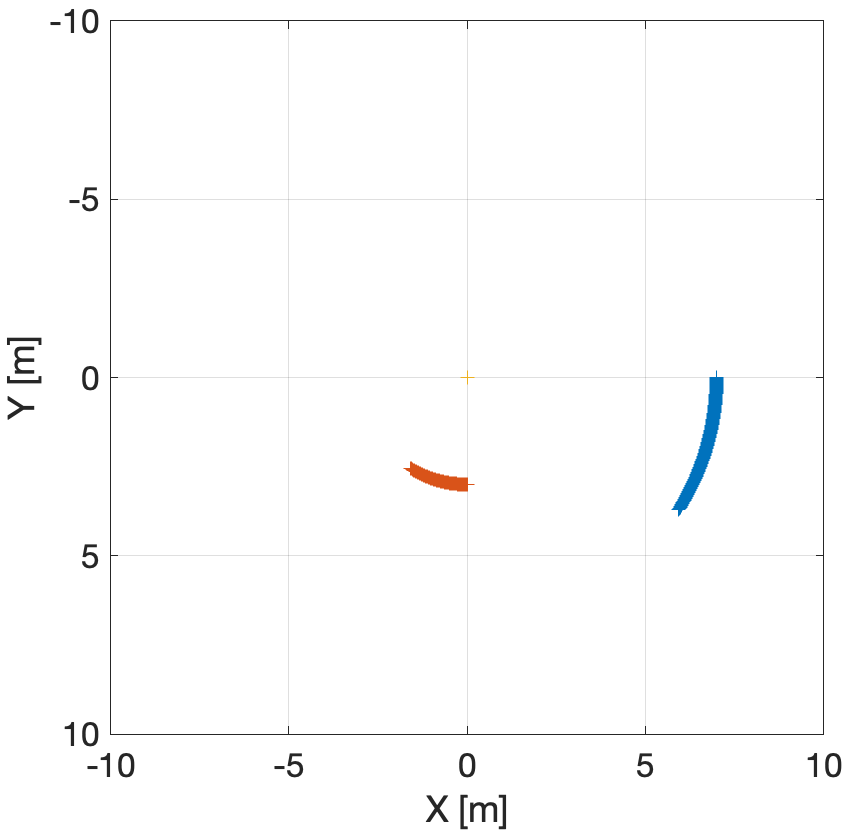
\includegraphics[width=0.3\linewidth]{Figures/traj.png}}%
    \label{fig:traj}
    \hfil
    \subfloat[]{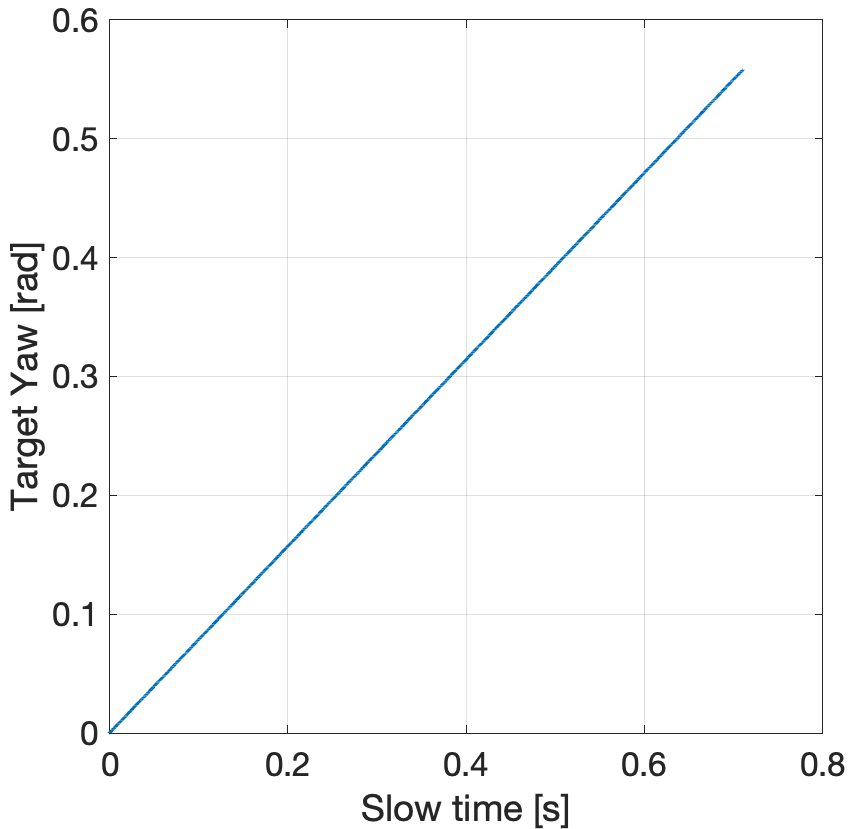
\includegraphics[width=0.3\linewidth]{Figures/yaws.png}}%
    \label{fig:yaws}
    \caption{(a.) The target range curves as a function of slow time. (b.) The target scattering point trajectories on an x-y plane. (c.) The orientation of the target as a function of slow time.}
\label{fig:target}
\end{figure*}

\subsection{Weighted backprojection} \label{sec:wbp}

In order to test the validity of the proposed compressed sensing-based methods, inspired by \cite{Zeng_2012, Tang_2016}, a weighted backprojection algorithm was implemented which weights the angular sampling per pulse. From Equation \ref{eq:wbp} and as depicted in Figure \ref{fig:nus}, the weighting can be defined as:
\begin{equation}
    W_{k} = \frac{\theta_{k+1} - \theta_{k-1}}{2}
    \label{eq:W}
\end{equation}

\noindent where $\theta_{k}$ is the angle ($\theta$) of the target at pulse $k$. In order to address the energy distortion caused by non-uniform sampling, the weighting in Equation \ref{eq:wbp} was normalized using the integration angle ($\theta_{\text{int}}$):

\begin{equation}
    w_{k} = W_{k} / \theta_{\text{int}}
\end{equation}

This methodology can also be applied to the backprojection algorithm described in Section \ref{sec:bp_la}. Both the interpolation matrix ($\psi_{in}$) and azimuth suppression matrix ($\psi_{bp}$) are formulated per pulse, allowing for the weighting to be applied in each block of $\psi_{in}$ or $\psi_{bp}$ per pulse.

\begin{figure}[H]
    \centering
    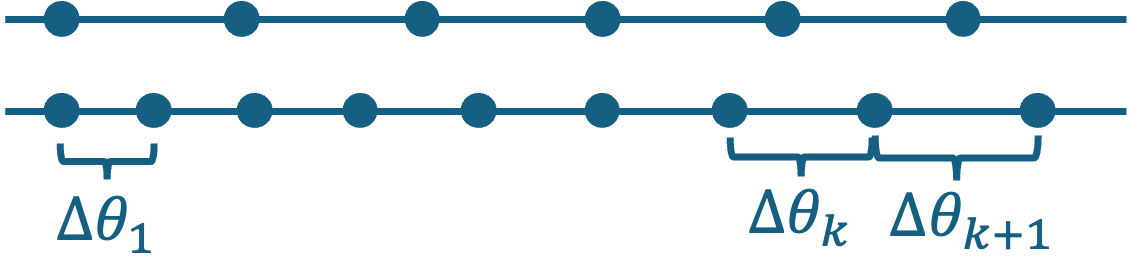
\includegraphics[width=0.8\linewidth]{Figures/nus.png}
    \caption{Non-uniform sampling}
    \label{fig:nus}
\end{figure}

\subsection{Compressed sensing for non-uniform sampling} \label{sec:bp_cs}

The weighted backprojection is able to compensate for the non-uniform rotation of targets and subsequent non-uniform sampling. However, by formulating the problem using a compressed sensing framework, non-uniform sampling can be viewed as an underdetermined system. This enables the utilization of compressed sensing techniques to improve the resolution of the image relative to the corrected backprojected image. Other methods interpolate from a non-uniform grid to a uniform grid as discussed in Section \ref{sec:intro}; however, these methods maintain the same number of samples and the same resolution. If the densest sampling corresponding to the beginning of the trajectory is used to define the desired sampling, the resolution of the image could be improved by estimating the gaps between the samples. Figure \ref{fig:nus_proposed} depicts the proposed sampling scheme where the points corresponding to gaps in sampling require estimation. 

\begin{figure}[H]
    \centering
    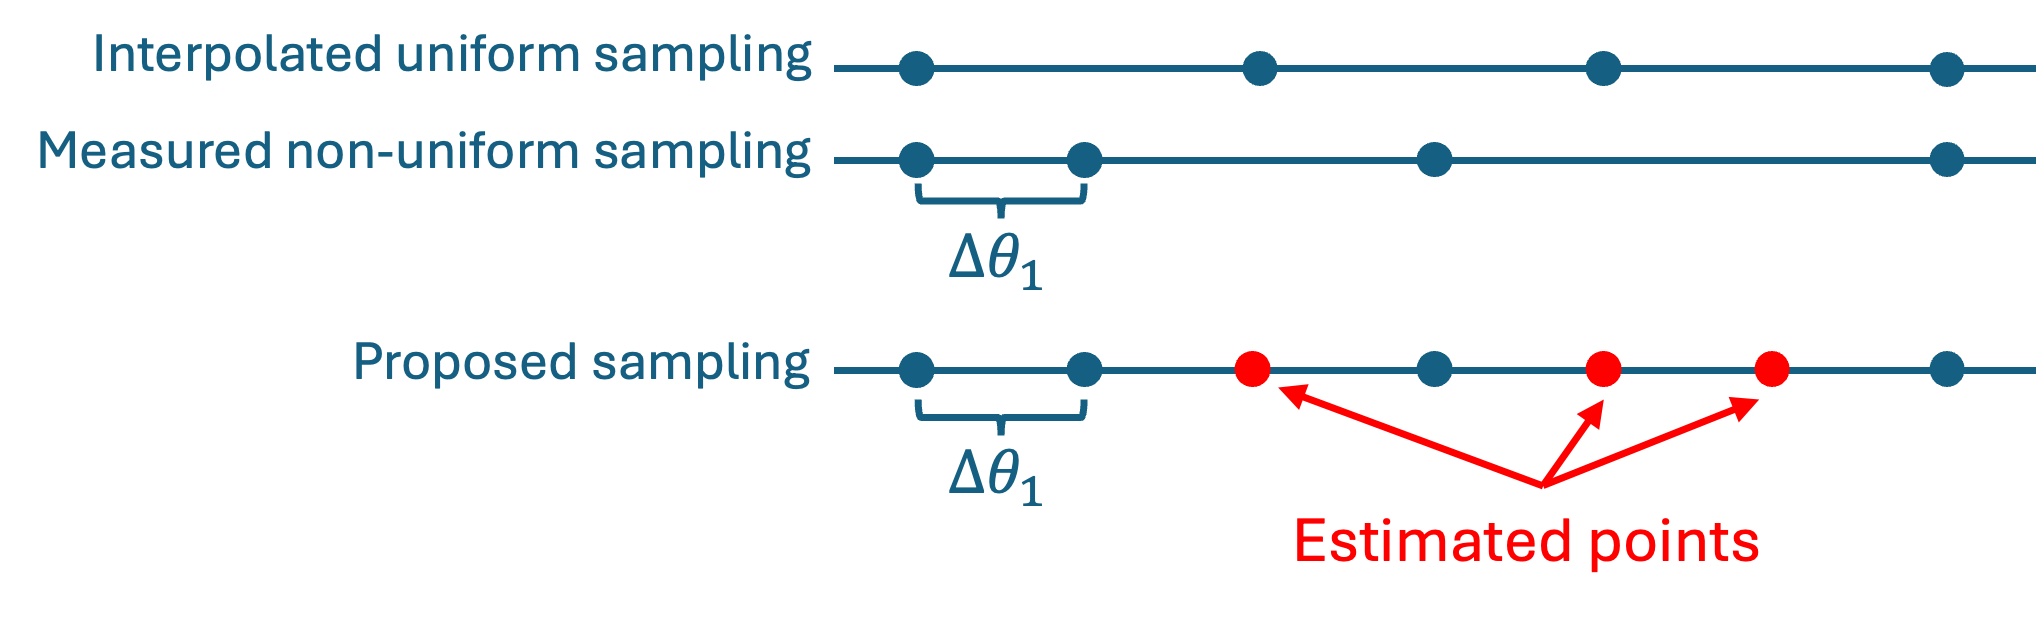
\includegraphics[width=0.9\linewidth]{Figures/nus_proposed.png}
    \caption{Non-uniform sampling with proposed estimation scheme}
    \label{fig:nus_proposed}
\end{figure}

From Equation \ref{eq:Ah}, the backprojection algorithm is defined as an explicit linear system where $x$ is the backprojected image, $A^{H}$ is the adjoint of the projection operator and $y$ is the measurement or ISAR image formed prior to azimuth compression. The backprojected image $x \in \mathbb{C}^{N}$ is deformed from non-uniform sampling and requires correction. A new linear system can be defined as:

\begin{equation}
    x = \tilde{A}\tilde{x} \label{eq:zAtx}
\end{equation}

\noindent where $\tilde{x} \in \mathbb{C}^{N}$ is the latent image with sampling estimation applied and $\tilde{A}$ is a sensing matrix which decomposes into a sparsifying transform ($\tilde{\psi} \in \mathbb{C}^{N \times N}$) and a measurement matrix ($\tilde{\phi} \in \mathbb{R}^{M \times N}$) as described in Equation \ref{eq:A}. The measurement matrix ($\tilde{\phi}$) applies non-uniform sampling to a fully-sampled latent image, producing a deformed measurement. With this linear equation, the OMP algorithm described in Algorithm \ref{algo:OMP} can be applied to estimate the latent image with super-resolution.



\section{Results}

% need:
% 1. image of target X
% 2. image comparing bp for la X
% 3. bp imaging table X
% 4. mse plots X
% 5. psf images X



\begin{figure*}[ht]
    \centering
    \subfloat[]{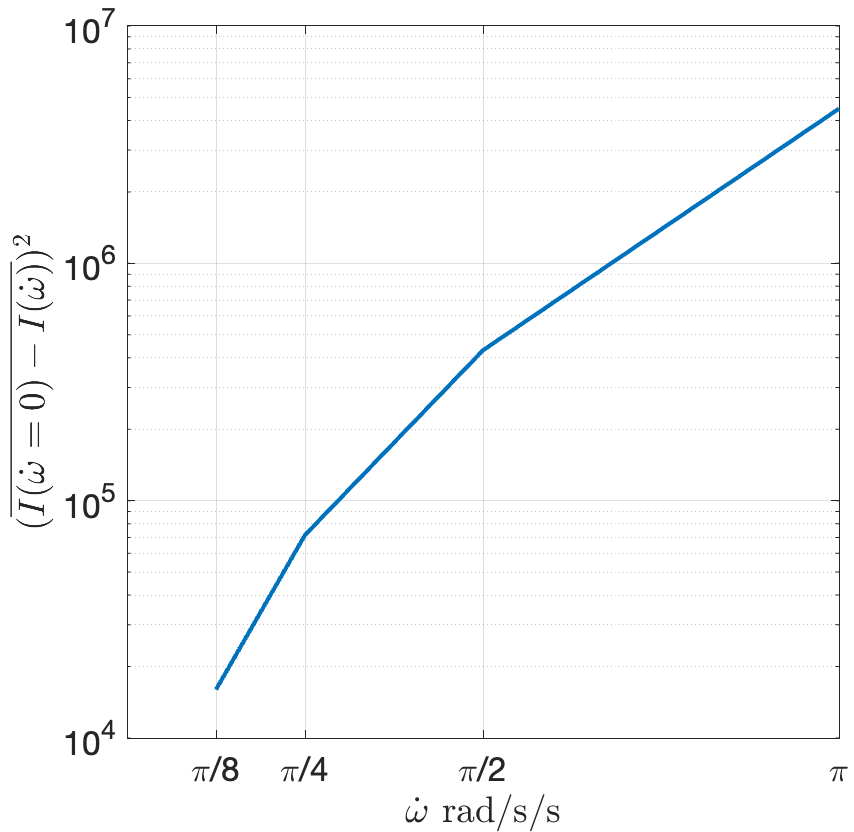
\includegraphics[width=0.3\linewidth]{Figures/mse_bp.png}}%
    \label{fig:range}
    \hfil
    \subfloat[]{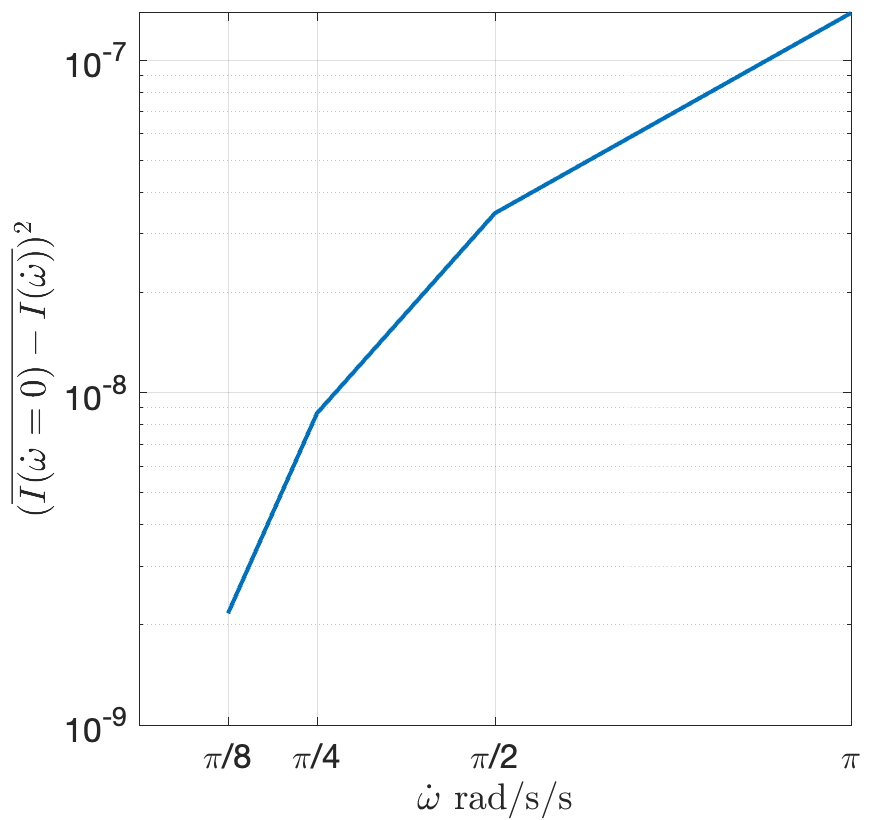
\includegraphics[width=0.3\linewidth]{Figures/mse_wbp.png}}%
    \label{fig:traj}
    \hfil
    \caption{Mean-squared error of a spatial domain image formed from (a.) the standard backprojection algorithm and from (b.) the weighted backprojection algorithm described in Section \ref{sec:wbp} with variable acceleration compared to a uniformly sampled image.}
\label{fig:mse}
\end{figure*}


To validate the efficacy of the methods described in Section \ref{sec:methods}, an ISAR imaging simulation was carried out using backprojection with a target containing three scatterers in an asymmetric configuration. The simulation was created in MATLAB with the target trajectory depicted in Figure \ref{fig:target} where the integration angle ($\theta$) is $32^{\circ}$ and the angular acceleration ($\alpha$) varies from $0$ rad/s/s to $2\pi$ rad/s/s. The target scattering points are confined to the $x-y$ plane, forming a tabletop simulation. The target is assumed to have perfect motion compensation in order to isolate the effects of non-uniform sampling. In order to ensure the images are formed with the same number of angular samples across all runs, the initial angular velocity is calculated using Equation \ref{eq:theta}:

\begin{equation}
    \begin{aligned}
        \theta &= \omega_{0} T + \frac{1}{2}\alpha T^{2} \\
        \rightarrow \omega_{0} &= \frac{1}{T} \left( \theta - \frac{1}{2}\alpha T^{2} \right)
    \label{eq:theta}
    \end{aligned}
\end{equation}

\noindent where the integration angle ($\theta$) is held constant across all simulation runs, $T$ is the simulation duration and $\alpha$ is the angular acceleration. Table \ref{tab:radar} depicts the radar parameters and the imaging parameters of the backprojection grid used for the simulation. From Section \ref{sec:bp_la}, the backprojection algorithm was formulated as an explicit linear system. Figure \ref{fig:bp_la} depicts a comparison of images formed using the methodology described in this section and the standard backprojection algorithm. The images are nearly identical, enabling for the utilization of compressed sensing techniques as the sensing matrix is directly derived. 

The results of imaging a non-uniformly rotating target without compensating for the non-uniform sampling is depicted in Figure \ref{fig:sd_sfd}. Figure \ref{fig:sd_sfd} highlights the impact of the non-uniform sampling on the energy distribution in k-space. As discussed in Section \ref{sec:intro}, as the angular sampling density is denser at the beginning of the target's trajectory relative to the end, the energy is concentrated at the beginning of the k-space support. As the angular acceleration increases, the deformation increases and more and more energy is re-distributed to the beginning of the k-space support. 

In contrast to the deformation visible in Figure \ref{fig:sd_sfd}, Figure \ref{fig:sd_sfd_w} depicts the results of implementing the weighted backprojection algorithm described in Section \ref{sec:wbp}. The normalized angular sampling weighting correctly re-distributes the energy uniformly across the k-space support. Furthermore, Figure \ref{fig:sd_sfd_w} also depicts the impact of the angular sampling density weighting on the image formation in the spatial domain. The deformation of the sidelobes is significantly reduced, and the results between the uniformly sampled image with $\dot{\omega} = 0$ rad/s/s are nearly identical to the image formed using the weighted backprojection with an angular acceleration of $\dot{\omega} = 2\pi$ rad/s/s. These results are emphasized in Figure \ref{fig:mse} where the mean-squared error is compared between the standard and weighted backprojection methods for varying angular acceleration. The shape of the two curves is similar; however, the magnitude of the error at $\dot{\omega} = 2\pi$ is on the order of $10^{6}$ for the standard implementation and $10^{-7}$ for the weighted implementation. This result is likely affected by the normalization described in Section \ref{sec:wbp}, and a more careful comparison is likely required.

\begin{table}[]
    \centering
    \begin{tabular}{|c|c|}
        \hline
        Parameter & Value \\ \hline 
        Center Frequency ($f_{c}$) & 1 GHz\\ \hline 
        Bandwidth ($B$) & 149.9 MHz \\ \hline
        Pulse Repetition Frequency & 10 kHz \\ \hline
        Sampling Frequency ($f_{s}$) & 600 MHz \\ \hline
        Pulse Width & $10 \mu s$ \\ \hline
        Backprojection Pixel Resolution [m] & 0.25 m \\ \hline
    \end{tabular}
    \caption{Radar and Imaging Parameters}
    \label{tab:radar}
\end{table}

\subsection{Compressed sensing for non-uniform sampling}

In order to demonstrate the effectiveness in estimating the gaps formed from non-uniform sampling, the methodology described in Section \ref{sec:bp_cs} was carried out on a frequency-domain signal ($\hat{x}\in\mathbb{C}^N$). From Equation \ref{eq:zAtx}, $\tilde{A} = \tilde{\Phi}\tilde{\Psi}$, where for this example, the frequency-domain signal $\hat{x}$ is assumed sparse in the time-domain ($x\in\mathbb{C}^N$), meaning the sparsifying transform is the inverse discrete Fourier Transform. This is a common assumption as the ISAR images depicted in Figures \ref{fig:sd_sfd} and \ref{fig:sd_sfd_w} are sparse in the spatial domain. The measurement matrix ($\tilde{\Phi} \in \mathbb{R}^{M \times N}$) was formed to reflect non-uniform sampling with a gradual increase in angular increment $\Delta\theta_{k}$ and $\Delta\theta_{1} \leq \Delta\theta_{k} \leq \Delta\theta_{M}$ as depicted in Figure \ref{fig:nus_proposed}. The measurement matrix is logical where values between angular samples were set to zero with $M$ non-zero values where $M < N$. Figure \ref{fig:cs_results} depicts a notional signal $x$ and its accompanying measurement $y \in \mathbb{R}^{M}$ with non-uniform sampling where $N = 200$ and $M = N/2$, as well as the fully sampled frequency-domain signal $\hat{x}$ and the compressed sensing approximation after applying OMP.

\begin{figure*}[ht]
    \centering
    \subfloat[]{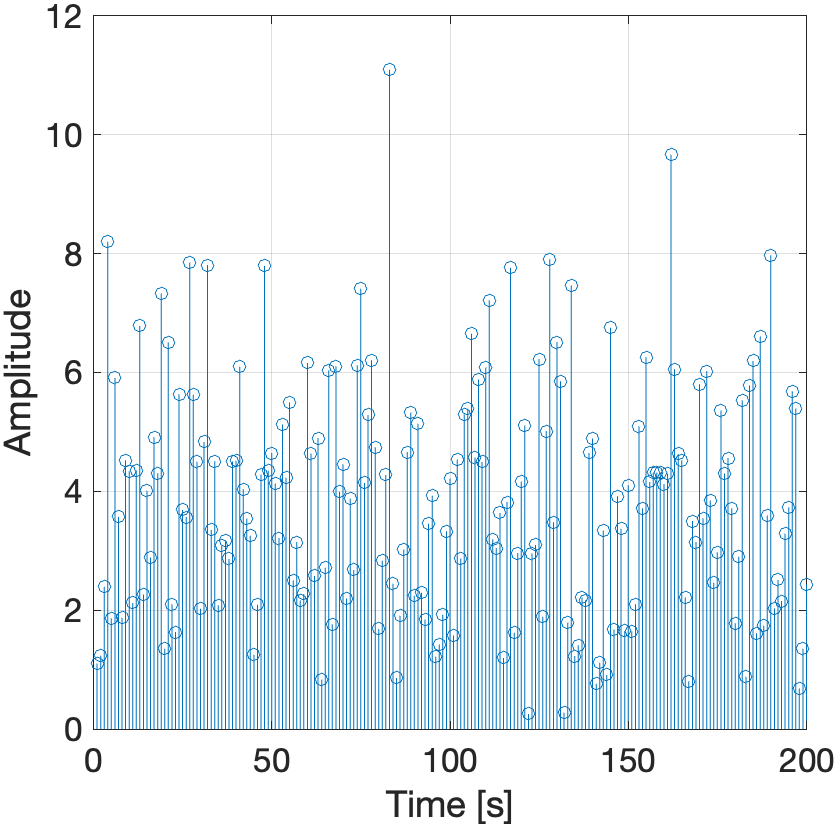
\includegraphics[width=0.2\linewidth]{Figures/x.png}}%
    \label{fig:range}
    \hfil
    \subfloat[]{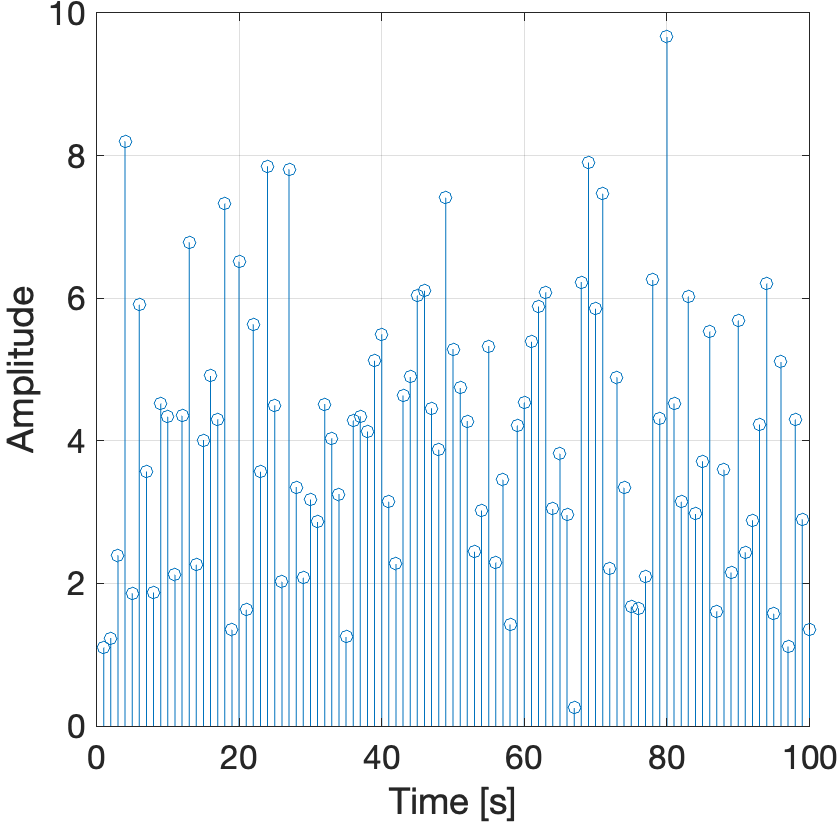
\includegraphics[width=0.2\linewidth]{Figures/y.png}}%
    \label{fig:traj}
    \hfil
    \subfloat[]{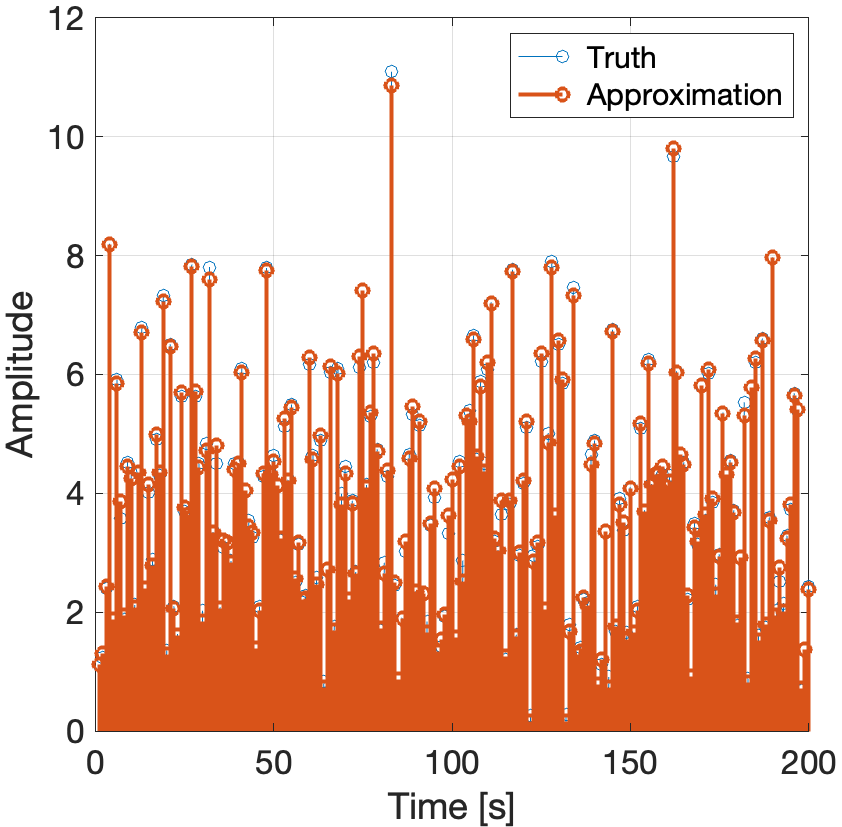
\includegraphics[width=0.2\linewidth]{Figures/recon_t.png}}%
    \label{fig:yaws}
    \hfil
    \subfloat[]{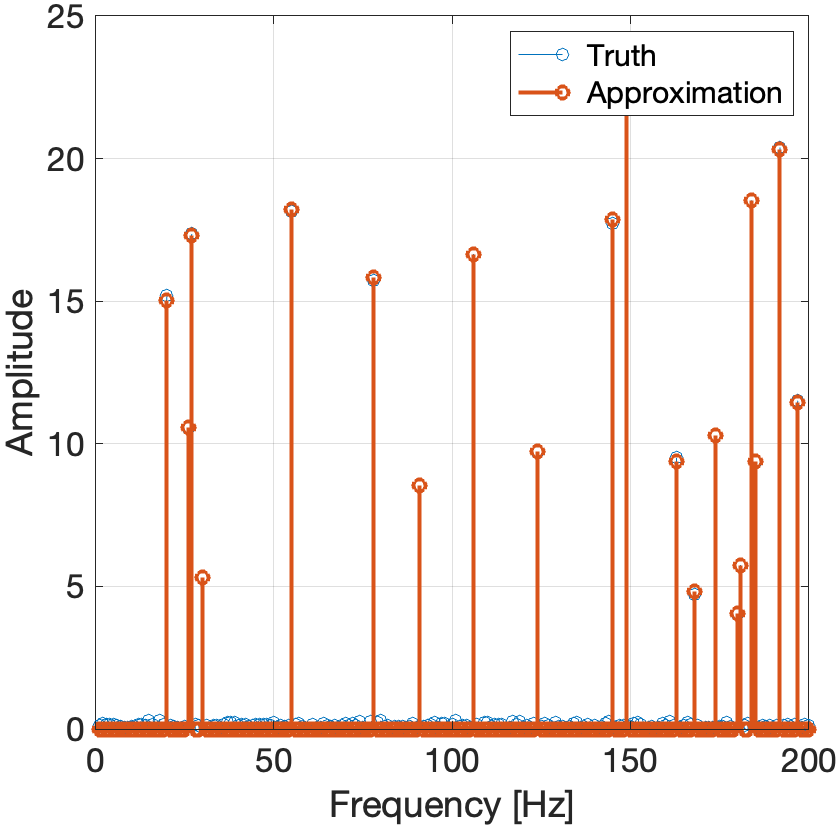
\includegraphics[width=0.2\linewidth]{Figures/recon_fft.png}}%
    \label{fig:yaws}
    \hfil
    \caption{(a.) The time-domain signal ($x$). (b.) The measurement time-domain signal ($y$). (c.) A comparison of the reconstruction and the truth data in the time-domain. (d.) A comparison of the reconstruction and the truth data in the frequency-domain.}
\label{fig:cs_results}
\end{figure*}

\section{Discussion}

\subsection{Representing backprojection as an explicit linear system}

From Figure \ref{fig:bp_la}, the implementation described in Section \ref{sec:bp_la} is able to form images by defining an explicit linear system. However, this implementation is computationally expensive for images of moderate size. The is a consequence of forming matrices of size $N_{x} \cdot N_{y} \cdot N_{p} \times N_{r}$ and $N_{x} \cdot N_{y} \times N_{x} \cdot N_{y} \cdot N_{p}$. The authors in \cite{Focsa_2021} recommend splitting the image into patches, and processing each patch individually. This modification will be required in the future to use the implementation described in Section \ref{sec:bp_la}.

\subsection{Weighted backprojection}

From Figure \ref{fig:sd_sfd_w}, the weighted backprojection model is able to form images of targets with non-uniform rotation and redistribute energy in k-space to match the image formed of a target rotating uniformly. This coincides with expectation as the weighting simply weights the contributions of each pulses as a function of the angular sampling density. The weighted backprojection model is able to reconstruct an image with perfect motion compensation and known angular samples, correcting distortions. This implementation is entirely dependent on weighting using angular samples which are typically derived from motion compensation. A next step would be formalizing the relationship between typical motion parameter estimation methods associated with motion compensation and the effects of non-uniform sampling. This would begin to determine if there is an optimal motion compensation/estimation method which is able to additionally prioritize compensating for non-uniform sampling.

\subsection{Compressed sensing for non-uniform sampling}

The results depicted in Figure \ref{fig:cs_results} demonstrate super-resolution reconstruction of a non-uniformly sampled signal. The methodology described in Section \ref{sec:bp_cs} is of a similar form as those derived in \cite{Liu_2012, Sun_2015, Zhang_2023}. However, these models deviate in either underlying image formation technique, sparsifying basis or resolution. A next step would be to apply this to the simulated ISAR image to verify the implementation's ability to reconstruct an image with non-uniform sampling at super-resolution. Additionally, more research must be done in comparing this methodology to other super-resolution and non-uniform reconstruction methodologies. Finally, the underlying compressed sensing technique (OMP) should be compared with state-of-the-art techniques involving machine learning and artificial intelligence, and the selection of the sparsifying basis should be more carefully scrutinized.  


\section{Conclusion}

The majority of ISAR imaging methods for a non-uniformly rotating target do not explicitly address non-uniform sampling. In order to produce images of targets with complex motion, the distortion caused by non-uniform sampling can be addressed directly by implementing a weighted backprojection. The weighted backprojection algorithm uses angular sampling weighting to remedy the non-uniform energy distribution in k-space and the distortion of the sidelobes in the spatial domain. Another potential avenue of addressing non-uniform sampling is compressed sensing, where the backprojection algorithm can be formulated as an explicit linear equation. Additionally, by defining a finer sampling grid, compressed sensing techniques can be used to "fill in the gaps", providing a higher resolution image. The intention of this article was to formalize much of the research and considerations given over the last couple of months. This article is not final and may not reflect the ultimate direction of the thesis, but hopefully provides some insight on the state of the problem and my research.

\printbibliography

%\begin{thebibliography}{00}
%\bibitem{b1} G. Eason, B. Noble, and I. N. Sneddon, ``On certain integrals of Lipschitz-Hankel type involving products of Bessel %functions,'' Phil. Trans. Roy. Soc. London, vol. A247, pp. 529--551, April 1955.
%\bibitem{b2} J. Clerk Maxwell, A Treatise on Electricity and Magnetism, 3rd ed., vol. 2. Oxford: Clarendon, 1892, pp.68--73.
%\bibitem{b3} I. S. Jacobs and C. P. Bean, ``Fine particles, thin films and exchange anisotropy,'' in Magnetism, vol. III, G. T. Rado and H. Suhl, Eds. New York: Academic, 1963, pp. 271--350.
%\bibitem{b4} K. Elissa, ``Title of paper if known,'' unpublished.
%\bibitem{b5} R. Nicole, ``Title of paper with only first word capitalized,'' J. Name Stand. Abbrev., in press.
%\bibitem{b6} Y. Yorozu, M. Hirano, K. Oka, and Y. Tagawa, ``Electron spectroscopy studies on magneto-optical media and plastic substrate interface,'' IEEE Transl. J. Magn. Japan, vol. 2, pp. 740--741, August 1987 [Digests 9th Annual Conf. Magnetics Japan, p. 301, 1982].
%\bibitem{b7} M. Young, The Technical Writer's Handbook. Mill Valley, CA: University Science, 1989.
%\end{thebibliography}

\end{document}
